%# -*- coding: utf-8-unix -*-
% !TeX spellcheck = zh_CN
\documentclass[oneside,UTF8,a4paper,12pt]{book}		% twoside 表示双面打印

\usepackage{url}
\usepackage{cite}
\usepackage{color}
\usepackage{xcolor}
\usepackage{import}
\usepackage{fancyhdr}
\usepackage{hyperref}								% 添加超链接
\usepackage{graphicx}
\usepackage{enumitem}
\usepackage{listings}								% 代码
\usepackage{transparent}
\usepackage{indentfirst}							% 段首缩进
\usepackage{supertabular}							% 长表格(换页处理)
\usepackage[utf8]{inputenc}
\usepackage[center]{titlesec}						% chapter1修改为第1章

\graphicspath{{./img/}}

\setlength{\parindent}{2em}							% 段首缩进
\setlength{\parskip}{.5em}							% 段落间距
\renewcommand{\baselinestretch}{1.3}				% 行间距

% 页眉
\pagestyle{fancy}
\renewcommand{\chaptermark}[1]{%
	\markboth{第\,\thechapter\,章\ #1}{}}

% 自定义命令

% 章节汉化
\titleformat{\chapter}{\raggedright\Huge\bfseries}{第\,\thechapter\,章}{1em}{}
\titleformat{\section}{\raggedright\Large\bfseries}{\,\thesection\,}{1em}{}
\titleformat{\subsection}{\raggedright\large\bfseries}{\,\thesubsection\,}{1em}{}
\titleformat{\subsubsection}{\raggedright\normalsize\bfseries}{\,\thesubsection\,}{1em}{}

% 目录居中
\renewcommand*\contentsname{\hfill 目录 \hfill}

% 设置itemize行间距
\setitemize{
	itemsep=0pt,
	partopsep=0pt,
	parsep=0.8em,
	topsep=5pt}
	
% 代码颜色设置
\definecolor{codegreen}{rgb}{0,0.6,0}
\definecolor{codegray}{rgb}{0.5,0.5,0.5}
\definecolor{codepurple}{rgb}{0.58,0,0.82}
\definecolor{backcolour}{rgb}{0.95,0.95,0.92}

\lstdefinestyle{mystyle}{
	backgroundcolor=\color{backcolour},   
	commentstyle=\color{codegreen},
	keywordstyle=\color{magenta},
	numberstyle=\tiny\color{codegray},
	stringstyle=\color{codepurple},
	basicstyle=\ttfamily\footnotesize,
	breakatwhitespace=false,         
	breaklines=true,                 
	captionpos=b,                    
	keepspaces=true,                 
	numbers=left,                    
	numbersep=5pt,                  
	showspaces=false,                
	showstringspaces=false,
	showtabs=false,                  
	tabsize=4
}
\lstset{style=mystyle}

% 定义
\newtheorem{note}{注意:}

% 去掉超链接红框
\hypersetup{hidelinks,
	colorlinks=true,
	allcolors=blue,
	pdfstartview=Fit,
	breaklinks=true}

\makeatletter
\def\UrlAlphabet{%
	\do\a\do\b\do\c\do\d\do\e\do\f\do\g\do\h\do\i\do\j%
	\do\k\do\l\do\m\do\n\do\o\do\p\do\q\do\r\do\s\do\t%
	\do\u\do\v\do\w\do\x\do\y\do\z\do\A\do\B\do\C\do\D%
	\do\E\do\F\do\G\do\H\do\I\do\J\do\K\do\L\do\M\do\N%
	\do\O\do\P\do\Q\do\R\do\S\do\T\do\U\do\V\do\W\do\X%
	\do\Y\do\Z}
\def\UrlDigits{\do\1\do\2\do\3\do\4\do\5\do\6\do\7\do\8\do\9\do\0}
\g@addto@macro{\UrlBreaks}{\UrlOrds}
\g@addto@macro{\UrlBreaks}{\UrlAlphabet}
\g@addto@macro{\UrlBreaks}{\UrlDigits}
\makeatother

% 字体
\usepackage{xeCJK}
\usepackage{graphicx}
\usepackage{fontspec} 
\setCJKmainfont{Source Han Mono SC} 


\begin{document}

\author{丁敬}
\title{X 教程}
\date{2023年04月26日}

\frontmatter										% 对前言和概览用罗马数字作为页码
\mainmatter      		 							% 对正文用阿拉伯数字作为页码
\maketitle
\tableofcontents									% 目录


\mainmatter
\begin{sloppypar}									% 自动换行
\chapter{新手开发者指南}

\section{X系统概念}

本章旨在向您介绍您需要了解的X窗口系统的基本概念和术语。当你有了这些概念,你将准备在后面的章节中更深入地研究特定的主题。

\subsection{X基于C/S结构}

X被设计成允许多个程序共享对一组公共硬件的访问。这种硬件既包括输入设备,如鼠标和键盘,也包括输出设备,如视频适配器和连接到它们的显示器。这些公共硬件由指定的某个进程进行统一管理,这个进程称为X服务端(因为它向客户机应用程序提供硬件设备的服务)。


与许多C/S系统一样,X服务端通常向许多同时运行的客户机提供服务,因此X服务端比大多数客户机运行的时间更长,并侦听来自新客户机的传入连接。


许多用户只在独立的笔记本电脑或桌面系统上使用X。在此设置中,X客户端与X服务器运行在同一台计算机上。然而,X为客户端/服务器通信定义了一个流协议。该协议可以通过网络公开,以允许客户端连接到不同机器上的服务器。这里需要注意的是,在这个模型中,客户机/服务器标签可能会令人困惑。此时在你面前的笔记本如果显示了远程机器客户端生成的图形,那么你当前的笔记本就是X服务端,生成图形的远程机器则是X客户端,如图 \ref{img-1.1.1-1}。


\begin{figure}[h]
    \centering
    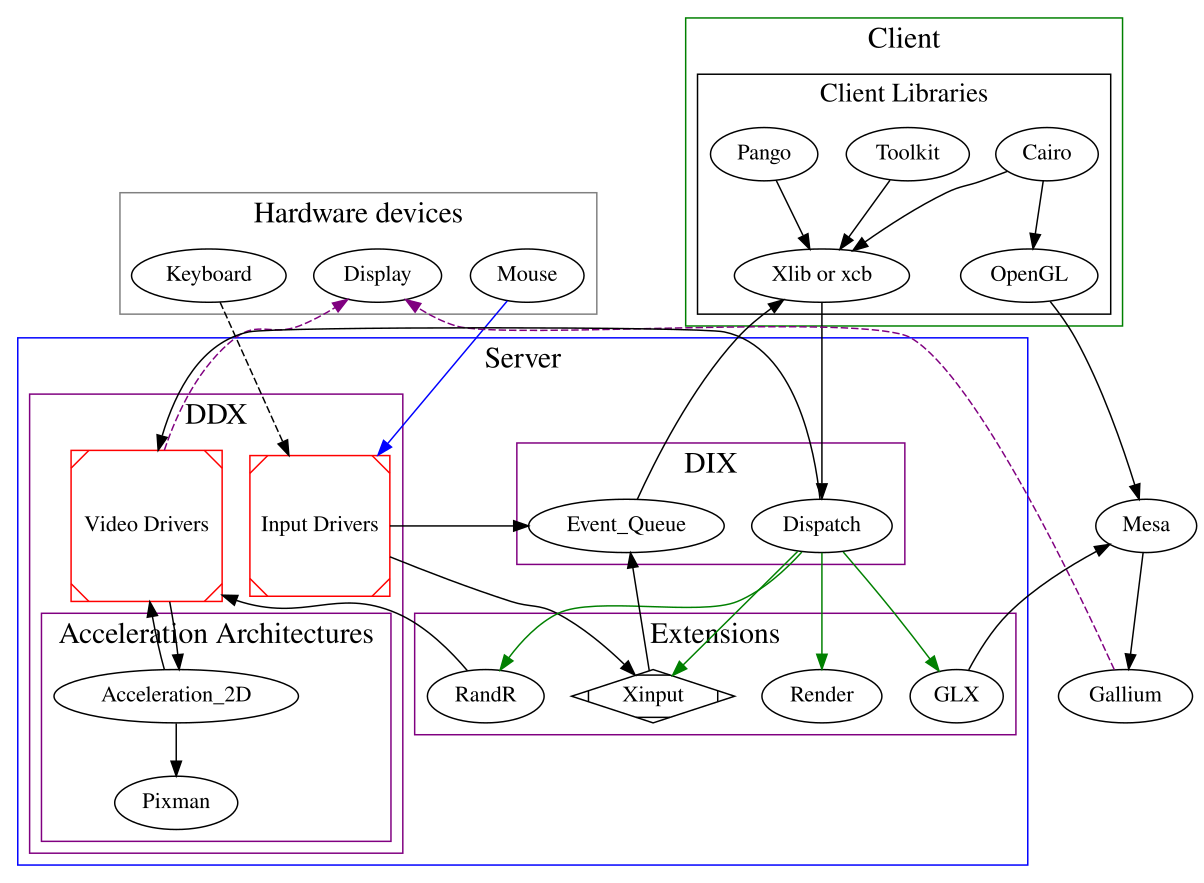
\includegraphics[scale=0.40]{x-1-1.png}
    \caption{X客户端/服务端模型}
    \label{img-1.1.1-1}
\end{figure}

\subsection{X实践}

本节描述X的一些基本组件及其工作原理。这个部分内容很多,有点像大杂烩。推荐的阅读方法是浏览一遍,然后回过头再读一遍。

\subsubsection{通过键盘输入}

X服务执行的任务之一是处理键盘上的输入,并将相应的键事件发送到适当的客户机应用程序。在简单的X配置中,每次只有一个客户端具有“输入焦点”,并且大多数关键事件将发送到该客户端。根据窗口管理器配置,只需将鼠标移动到另一个窗口、单击鼠标、使用热键或操作显示可用客户机的面板,就可以将焦点移动到另一个窗口。具有焦点的客户端通常以某种方式突出显示,以便用户可以知道他们的输入将流向何处。客户端可以使用“抓取”(在本章后面描述)来覆盖向重点客户端发送关键事件的默认交付。


\chapter{Xlib}


\section{xlib简介}

X的前10个版本的设计和实现主要是由三个人完成的:麻省理工学院计算机科学实验室的罗伯特·舍弗勒、数字设备公司的吉姆·盖提斯和麻省理工学院的罗恩·纽曼,他们都是麻省理工学院雅典娜项目的成员。然而,X的第11个版本则是许多地方和组织共同努力的成果。

X窗口系统是麻省理工学院设计的一个网络透明窗口系统。X显示服务器运行在具有单色或彩色位图显示硬件的计算机上。服务器将用户输入分发给位于同一台机器上或网络中其他地方的各种客户机程序,并接受它们的输出请求。Xlib是一个C子例程库,应用程序(客户端)使用它通过流连接与窗口系统进行交互。尽管客户机通常运行在与其通信的X服务器所在的同一台机器上,但情况并非如此。

Xlib−C语言X接口是X窗口系统协议的低级C语言接口的参考指南。它既不是教程,也不是X窗口系统编程的用户指南。相反,它提供了库中每个函数的详细描述以及相关背景信息的讨论。Xlib−C语言X界面假定对图形窗口系统和C编程语言有基本的了解。其他高级抽象(例如,由X工具包提供的抽象)构建在Xlib库之上。有关这些高级库的进一步信息,请参阅相应的工具包文档。X窗口系统协议(Window System Protocol)\footnote{\url{https://www.x.org/releases/current/doc/}}提供了关于X的行为的权威词汇。尽管这里出现了额外的信息,但协议文档是主导文档。

\subsection{X窗口系统概述}

本书中使用的一些术语是X所独有的,而其他窗口系统通用的其他术语在X中具有不同的含义。您可能会发现参考位于本书末尾的术语表会有所帮助。

X窗口系统支持一个或多个包含重叠窗口或子窗口的屏幕。屏幕是一个物理显示器和硬件,可以是彩色、灰度或单色的。每个显示器或工作站可以有多个屏幕。单个X服务器可以为任意数量的屏幕提供显示服务。单个用户使用一个键盘和一个指针(通常是鼠标)的一组屏幕称为显示器。

X服务器中的所有窗口都按照严格的层次结构进行安排。在每个层次结构的顶部是一个根窗口,它覆盖了每个显示屏幕。每个根窗口部分或全部被子窗口覆盖。除根窗口外,所有窗口都有父窗口。通常每个应用程序至少有一个窗口。子窗口可能会有自己的子窗口。通过这种方式,应用程序可以在每个屏幕上创建任意深度的树。X为窗口提供图形、文本和光栅操作。

子窗口可以比父窗口大。也就是说,子窗口的部分或全部可以扩展到父窗口的边界之外,但是窗口的所有输出都被其父窗口剪切。如果一个窗口的几个子窗口有重叠的位置,则认为其中一个子窗口位于其他子窗口之上或高于其他子窗口,从而使它们变得模糊。输出到其他窗口覆盖的区域将被窗口系统抑制,除非该窗口具有后备存储。如果一个窗口被第二个窗口遮挡,第二个窗口只遮挡第二个窗口的祖先,同时也是第一个窗口的祖先。

窗口的边框宽度为0或更多像素,可以是任何图案(像素图)或您喜欢的纯色。一个窗口通常(但不总是)有一个背景图案,当被揭开时,它将被窗口系统重新绘制。子窗口掩盖了父窗口,父窗口中的图形操作通常由子窗口剪切。

每个窗口和像素图都有自己的坐标系统。坐标系的X轴为水平轴,Y轴为垂直轴,原点[0,0]位于左上角。坐标是积分的,以像素为单位,并与像素中心重合。对于窗口,原点在内部左上角的边界内。

X不保证保留窗口的内容。当一个窗口的部分或全部被隐藏,然后再回到屏幕上,它的内容可能会丢失。然后,服务器向客户端程序发送一个Expose事件,通知它需要重新绘制部分或全部窗口。程序必须准备好在需要时重新生成窗口的内容。

X还提供图形对象的屏幕外存储,称为pixmaps。单平面(深度为1)像素图有时被称为位图。像素图可以在大多数图形函数中与窗口互换使用,并在各种图形操作中用于定义模式或块。窗口和像素图一起被称为可绘制图。

Xlib中的大多数函数只是将请求添加到输出缓冲区。这些请求稍后在X服务器上异步执行。返回存储在服务器中的信息值的函数在接收到显式回复或发生错误之前不会返回(也就是说,它们会阻塞)。您可以提供一个错误处理程序,它将在报告错误时被调用。

如果客户端不希望请求异步执行,它可以在请求之后调用XSync,该调用将阻塞,直到所有先前缓冲的异步事件都被发送并执行。作为一个重要的副作用,Xlib中的输出缓冲区总是在调用任何从服务器返回值或等待输入的函数时被刷新。

许多Xlib函数将返回一个整数资源ID,它允许您引用存储在X服务器上的对象。这些类型可以是Window、Font、Pixmap、Colormap、Cursor和GContext,如文件<X11/X.h>中定义的。这些资源由请求创建,并在请求或连接关闭时销毁(或释放)。这些资源中的大多数都可能在应用程序之间共享,事实上,窗口是由窗口管理器程序显式地操纵的。字体和游标在多个屏幕之间自动共享。字体根据需要加载和卸载,并由多个客户端共享。字体通常缓存在服务器中。Xlib不支持在应用程序之间共享图形上下文。

客户端程序被告知事件。事件可能是请求的副作用(例如,重新堆叠窗口生成Expose事件),也可能是完全异步的(例如,来自键盘)。客户端程序要求获得事件通知。由于其他应用程序可以向您的应用程序发送事件,因此程序必须准备好处理(或忽略)所有类型的事件。

输入事件(例如,按下键或指针移动)从服务器异步到达,并排队,直到显式调用(例如,XNextEvent或XWindowEvent)请求它们。此外,一些库函数(例如XRaiseWindow)会生成Expose和ConfigureRequest事件。这些事件也是异步到达的,但是客户机可能希望在调用一个函数之后通过调用XSync显式地等待它们,该函数会导致服务器生成事件。

\subsection{错误}

一些函数返回Status(一个表示错误信息的整数)。如果函数失败,则返回0。如果函数返回状态为0,则表示它没有更新返回参数。由于C语言不提供多个返回值,因此许多函数必须通过写入客户端传递的存储来返回结果。默认情况下,错误由标准库函数或您提供的函数处理。如果字符串不存在,返回指向字符串指针的函数返回NULL指针。

X服务器在检测到协议错误时候就会报告错误信息。如果一个给定的请求可以生成多个错误,服务器可以报告其中的任何一个。

由于Xlib通常不会立即将请求传输到服务器(也就是说,它会缓冲请求),因此报告错误的时间可能比实际发生的时间晚得多。然而,出于调试目的,Xlib提供了一种强制同步行为的机制(参见11.8.1节)。当启用同步时,错误会在生成时报告。

当Xlib检测到错误时,它调用程序可以提供的错误处理程序。如果不提供错误处理程序,则打印错误并终止程序。

\subsection{标准头文件}

\begin{itemize}
	\item <X11/Xlib.h>:这是Xlib的主要头文件。大多数Xlib符号都是通过包含这个文件来声明的。该文件还包含预处理器符号XlibSpecificationRelease。此符号在本标准中定义为6。(Xlib的第5版是第一个有这个符号的版本。)
	\item <X11/X.h>:该文件声明了应用程序将使用的X协议的类型和常量。它从<X11/Xlib.h>自动包含,因此应用程序代码不需要直接引用该文件。
	\item <X11/Xcms.h>:这个文件包含了第6章中描述的许多颜色管理工具的符号。所有以“Xcms”为前缀的函数、类型和符号,以及颜色转换上下文宏,都在这个文件中声明。在包含此文件之前必须包含<X11/Xlib.h>。
	\item <X11/Xutil.h>:该文件声明了用于客户端间通信和应用程序实用程序的各种函数、类型和符号,这些将在第14章和第16章中描述。在包含此文件之前必须包含<X11/Xlib.h>。
	\item <X11/Xresource.h>:该文件声明了资源管理器设施的所有函数、类型和符号,这些将在第15章中描述。在包含此文件之前必须包含<X11/Xlib.h>。
	\item <X11/Xatom.h>:该文件声明了所有预定义的原子,这些原子是前缀为“XA\_”的符号。
	\item <X11/cursorfont.h>:该文件声明了标准游标字体的游标符号,它们列在附录b中。所有的游标符号都有前缀“XC\_”。
	\item <X11/keysymdef.h>:该文件声明了所有标准KeySym值,这些值是前缀为“XK\_”的符号。键盘系统按组排列,预处理器符号控制每组的包含。必须在包含文件之前定义预处理器符号以获得相关值。预处理器符号是xk\_miscellaneous, XK\_XKB\_KEYS, XK\_3270, XK\_LATIN1, XK\_LATIN2, XK\_LATIN3, XK\_LATIN4, XK\_KATAKANA, XK\_ARABIC, XK\_CYRILLIC, XK\_GREEK, XK\_TECHNICAL, XK\_SPECIAL, XK\_PUBLISHING, XK\_APL, XK\_HEBREW, XK\_THAI和XK\_KOREAN。
	\item <X11/keysym.h>:这个文件定义了预处理器符号xk\_miscellaneous, XK\_XKB\_KEYS, XK\_LATIN1, XK\_LATIN2, XK\_LATIN3, XK\_LATIN4和XK\_GREEK,然后包括<X11/keysymdefh>。
	\item <X11/Xlibint.h>:该文件声明了用于扩展的所有函数、类型和符号,这些在附录c中有描述。该文件自动包含<X11/Xlib.h>。
	\item <X11/Xproto.h>:该文件声明了基本X协议的类型和符号,以便在实现扩展时使用。它从<X11/xlibin.h>自动包含,因此应用程序和扩展代码不需要直接引用该文件。
	\item <X11/Xprotostr.h>:该文件声明了基本X协议的类型和符号,以便在实现扩展时使用。它从<X11/xproto1.h>自动包含,因此应用程序和扩展代码不需要直接引用该文件。
	\item <X11/X10.h>:该文件声明了用于X10兼容性函数的所有函数、类型和符号,这些在附录D中有描述。
\end{itemize}

\subsection{常用值和类型}

\noindent 以下符号由Xlib定义,并在整个手册中使用:
\begin{itemize}
	\item Xlib定义Bool类型和布尔值True和False。
	\item None是通用的空资源ID或原子。
	\item 类型XID用于通用资源id。
	\item 类型XPointer定义为char*,并用作指向数据的泛型不透明指针。
\end{itemize}

\subsection{Xlib中的命名和参数约定}

Xlib在函数的命名和语法方面遵循许多约定。假设您记住了函数需要的信息,这些约定旨在使函数的语法更加可预测。

\noindent 主要的命名约定有:

\begin{itemize}
	\item 为了将X符号与其他符号区分开来,库对外部符号使用混合大小写。按照现有约定,它为变量保留小写字母,为用户宏保留全部大写字母。
	\item 所有Xlib函数都以大写X开头。
	\item 所有函数名和符号的开头都大写。
	\item 所有用户可见的数据结构都以大写X开头。更一般地说,用户可以解引用的任何内容都以大写X开头。
	\item 宏和其他符号不以大写x开头。为了区别于所有用户符号,宏中的每个单词都大写。
	\item 数据结构中的所有元素或变量都是小写的。必要时,复合词用下划线(\_)构成。
	\item 当使用display参数时,它总是在参数列表的第一个。
	\item 所有使用的资源对象都出现在参数列表的开头,紧跟在display参数之后。
	\item 当图形上下文与另一种类型的资源(最常见的是可绘制的资源)一起出现时,图形上下文出现在参数列表中,位于其他资源之后。可抽取资源的排名高于所有其他资源。
	\item 在参数列表中,源参数总是位于目标参数之前。
	\item 在参数列表中,x参数总是位于y参数之前。
	\item 在参数列表中,宽度参数总是位于高度参数之前。
	\item 当x、y、width和height参数一起使用时,x和y参数总是在width和height参数之前。
	\item 当掩码与结构体同时出现时,掩码总是位于参数列表中指向该结构体的指针之前。
\end{itemize}

\subsection{编程注意事项}

\noindent 主要的编程考虑是:

\begin{itemize}
	\item X中的坐标和大小实际上是16位的量。这个决定是为了最小化给定性能级别所需的带宽。坐标通常在接口中声明为int。大于16位的值将被静默截断。尺寸(宽度和高度)被声明为无符号数量。
	\item 键盘是不同制造商工作站之间最大的变量。如果你希望你的程序是可移植的,你应该在这里特别保守。
	\item 许多显示系统的屏幕外内存有限。如果可以的话,应该尽量减少像素图和后备存储的使用。
	\item 用户应该能够控制自己的屏幕空间。因此,您应该编写应用程序来响应窗口管理,而不是假定控制整个屏幕。但是,在顶层窗口内执行的操作取决于应用程序。有关更多信息,请参阅第14章和客户端间通信约定手册。
\end{itemize}

\subsection{字符集和编码}

\noindent 一些Xlib函数引用了特定的字符集和字符编码。以下是最常见的:

\subsubsection{x可移植字符集(X Portable Character Set)}

97个字符的基本集合,假定存在于Xlib支持的所有语言环境中。该字符集包含以下字符:

\begin{lstlisting}
a..z
A..Z
0..9
!"#$\%&'()*+,-./:;<=>?@[\\]^_`{|}~
<space>, <tab>, <newline>
\end{lstlisting}

该字符集是ISO8859-1图形字符集的左/下半部分加上空格、制表符和换行符。它也是7位ASCII的图形字符集加上相同的三个控制字符。这些字符在主机上的实际编码取决于系统。

\subsubsection{主机可移植字符编码}

主机上X可移植字符集的编码。编码本身不是由这个标准定义的,但是在主机上Xlib支持的所有语言环境中,编码必须是相同的。如果一个字符串被称为主机可移植字符编码,那么它只包含来自主机编码的X可移植字符集的字符。

\subsubsection{Latin-1}

由ISO8859-1标准定义的编码字符集。

\subsubsection{Latin可移植字符编码}

使用Latin-1码点加上ASCII控制字符对X可移植字符集进行编码。如果一个字符串被称为Latin Portable Character Encoding,那么它只包含来自X Portable Character Set的字符,而不是Latin-1的所有字符。

\subsubsection{STRING编码}

Latin-1,加上制表符和换行符。

\subsubsection{POSIX可移植文件名字符集}

65个字符的集合,可用于在posix兼容的主机上命名文件,在所有语言环境中都能正确处理。集合为:


\begin{lstlisting}
a..z
A..Z
0..9
._-
\end{lstlisting}

\subsubsection{格式规范}

\noindent Xlib−C语言X接口使用以下约定:

\begin{itemize}

\item 全局符号以这种特殊字体打印。这些可以是函数名、包含文件中定义的符号或结构名。在声明和定义时,函数参数以斜体打印。在后面的解释性文字中,它们通常是用普通字体打印的。
\item 每个函数都是通过一般性讨论来介绍的,以区别于其他函数。函数声明本身紧随其后,并对每个参数进行了具体解释。虽然没有使用ANSI C函数原型语法,但Xlib头文件通常使用ANSI C环境中的函数原型来声明函数。如果需要对函数进行一般性讨论,则在参数之后进行。在适用的情况下,说明的最后一段列出了函数可能生成的Xlib错误码。有关Xlib错误码的完整讨论,请参见第11.8.2节。
\item 为了消除您传递的参数和函数返回给您的参数之间的任何歧义,您传递的所有参数的解释都以单词specify开头,或者在有多个参数的情况下,以单词specify开头。返回给您的所有参数的解释都以单词returns开头,或者在有多个参数的情况下,以单词return开头。您可以传递和返回的所有参数的解释都以单词指定和返回开始。
\item 任何指向用于返回值的结构体的指针都由\_return后缀作为其名称的一部分指定。传递给这些函数的所有其他指针仅用于读取。一些参数使用指向结构体的指针,这些结构体同时用于输入和输出,并使用\_in\_out后缀表示。
\end{itemize}

\section{显示(Display)相关函数}

\noindent 在您的程序可以使用显示器之前,您必须建立到X服务器的连接。一旦建立了连接,就可以使用本章讨论的Xlib宏和函数来返回有关显示的信息。本章讨论以下几点:

\begin{itemize}
	\item 打开(连接到)显示器
	\item 获取有关显示、图像格式或屏幕的信息
	\item 生成一个NoOperation协议请求
	\item 释放客户端创建的数据
	\item 关闭(断开)显示器
	\item 使用X服务器关闭连接操作
	\item 使用带有线程的Xlib
	\item 使用内部连接
\end{itemize}

\subsection{打开显示器}

要打开到控制显示的X服务器的连接,请使用XOpenDisplay。

\begin{lstlisting}[language=C]
	Display* XOpenDisplay(char* display_name);
\end{lstlisting}

\begin{note}
	display\_name: 指定硬件显示名称,该名称确定要使用的显示和通信域。在符合posix的系统上,如果display\_name为NULL,则默认为DISPLAY环境变量的值。
\end{note}

XOpenDisplay函数返回一个Display结构,该结构用作到X服务器的连接,并且包含关于该X服务器的所有信息。XOpenDisplay通过TCP或DECnet通信协议,或通过某些本地进程间通信协议,将应用程序连接到X服务器。如果协议指定为“tcp”、“inet”或“inet6”,或者没有指定协议,主机名是主机名,主机名和显示号之间用一个冒号分隔,XOpenDisplay使用tcp流连接。(如果指定的协议为“inet”,则使用TCP over IPv4。如果指定协议为inet6,则使用TCP over IPv6。否则,实现将决定使用哪个IP版本。)如果没有指定主机名和协议,Xlib将使用它认为最快的传输方式。如果主机名是主机名,用双冒号(::)分隔主机名和显示号,XOpenDisplay使用DECnet进行连接。单个X服务器可以同时支持任何或所有这些传输机制。特定的Xlib实现可以支持更多这样的传输机制。

如果成功,XOpenDisplay返回一个指向Display结构的指针,该结构在<X11/Xlib.h>中定义。如果XOpenDisplay不成功,它返回NULL。在成功调用XOpenDisplay之后,客户机可以使用显示中的所有屏幕。display\_name参数中指定的屏幕编号由DefaultScreen宏(或XDefaultScreen函数)返回。只能通过使用信息宏或函数来访问Display和Screen结构的元素。有关使用宏和函数从Display结构中获取信息的信息,请参见2.2.1节。

\subsection{获取有关显示、图像格式或屏幕的信息}

Xlib库提供了许多有用的宏和相应的函数,它们从Display结构返回数据。这些宏用于C编程,它们对应的函数等价于其他语言绑定。本节讨论:

\begin{itemize}
	\item 显示宏
	\item 图像格式函数和宏
	\item 屏幕信息宏
\end{itemize}

Display结构的所有其他成员(即没有为其定义宏的成员)都是Xlib私有的,不能使用。应用程序绝对不能直接修改或检查Display结构的这些私有成员。下一节中的XDisplayWidth、XDisplayHeight、XDisplayCells、XDisplayPlanes、XDisplayWidthMM和XDisplayHeightMM函数命名不当。这些函数应该命名为Screenwhatever和XScreenwhatever,而不是Displaywhatever或XDisplaywhatever。对于由此造成的混乱,我们深表歉意。

\subsubsection{Display Macros}

应用程序不应该直接修改Display和Screen结构的任何部分。这些成员应该被认为是只读的,尽管它们可能会由于对显示的其他操作而改变。下面列出了C语言的宏,它们对应的用于其他语言绑定的等价函数,以及它们都可以返回的数据。

\begin{lstlisting}[language=C]
unsigned long XAllPlanes(void);
unsigned long XBlackPixel(Display *display, int screen_number);
unsigned long XWhitePixel(Display *display, int screen_number);
int XConnectionNumber(Display *display);
Colormap XDefaultColormap(Display *display, int screen_number);
int XDefaultDepth(Display *display, int screen_number);
int *XListDepths(Display *dsp, int screen_num, int* count_ret);
GC XDefaultGC(Display *display, int screen_number);
Window XDefaultRootWindow(Display *display);
Screen *XDefaultScreenOfDisplay(Display *display);
Screen *XScreenOfDisplay(Display *display, int screen_number);
int XDefaultScreen(Display *display);
Visual *XDefaultVisual(Display *display, int screen_number);
int XDisplayCells(Display *display, int screen_number);
int XDisplayPlanes(Display *display, int screen_number);
char *XDisplayString(Display *display);
long XExtendedMaxRequestSize(Display *display);
long XMaxRequestSize(Display *display);
unsigned long XLastKnownRequestProcessed(Display *display);
unsigned long XNextRequest(Display *display);
int XProtocolVersion(Display *display);
int XProtocolRevision(Display *display);
int XQLength(Display *display);
Window XRootWindow(Display *display, int screen_number);
int XScreenCount(Display *display);
char *XServerVendor(Display *display);
int XVendorRelease(Display *display);
\end{lstlisting}

\subsubsection{图像格式函数和宏}

应用程序需要以服务器要求的格式向X服务器提供数据。为了帮助简化应用程序,转换数据所需的大部分工作都由Xlib提供(参见第8.7和16.8节)。

XPixmapFormatValues结构提供了在连接建立时返回的像素图格式信息的接口。它包含:

\begin{lstlisting}[language=C]
typedef struct {
	int depth;
	int bits_per_pixel;
	int scanline_pad;
} XPixmapFormatValues;
\end{lstlisting}

\noindent 要获取给定显示的像素图格式信息,请使用XListPixmapFormats,其中 count\_return 表示:返回显示所支持的像素图格式的数目。

\begin{lstlisting}[language=C]
XPixmapFormatValues* XListPixmapFormats(
	Display* display,
	int* count_return);
\end{lstlisting}

\noindent XListPixmapFormats函数返回一个XPixmapFormatValues结构数组,这些结构描述了指定显示所支持的Z格式图像的类型。如果可用内存不足,XListPixmapFormats返回NULL。要为XPixmapFormatValues结构释放已分配的存储空间,请使用XFree。

\noindent 下面列出了C语言宏、它们对应的用于其他语言绑定的等价函数,以及它们为指定的服务器和屏幕返回的数据。这些通常被工具包和简单的应用程序使用。

\begin{lstlisting}[language=C]
int XImageByteOrder(Display *display);
\end{lstlisting}

\noindent 两者都为XY格式(位图)的每个扫描线单元或Z格式的每个像素值指定图像所需的字节顺序。宏或函数可以返回LSBFirst或MSBFirst。
\begin{lstlisting}[language=C]
int XBitmapUnit(Display *display);
\end{lstlisting}

\noindent 两者都以位为单位返回位图扫描线的大小。扫描线以该值的倍数计算。
\begin{lstlisting}[language=C]
int XBitmapBitOrder(Display *display);
\end{lstlisting}

\noindent 在每个位图单元中,屏幕上显示的位图中最左边的位要么是该单元中最不重要的位,要么是最重要的位。这个宏或函数可以返回LSBFirst或MSBFirst。
\begin{lstlisting}[language=C]
int XBitmapPad(Display *display);
\end{lstlisting}

\noindent 每个扫描线必须填充为该宏或函数返回的位的倍数。
\begin{lstlisting}[language=C]
int XDisplayHeight(Display *display, int screen_number);
\end{lstlisting}

\noindent 两者都返回一个以像素为单位描述屏幕高度的整数。
\begin{lstlisting}[language=C]
int XDisplayHeightMM(Display *display, int screen_number);
\end{lstlisting}

\noindent 以下都是返回屏幕宽度。
\begin{lstlisting}[language=C]
int XDisplayWidth(Display *display, int screen_number);
int XDisplayWidthMM(Display *display, int screen_number);
\end{lstlisting}

\subsubsection{屏幕信息宏}

\noindent 下面列出了C语言宏,它们对应的用于其他语言绑定的等价函数,以及它们都可以返回的数据。这些宏或函数都有一个指向适当屏幕结构的指针。
\begin{lstlisting}[language=C]
unsigned long XBlackPixelOfScreen(Screen *screen);
unsigned long XWhitePixelOfScreen(Screen *screen);
int XCellsOfScreen(Screen *screen);
Colormap XDefaultColormapOfScreen(Screen *screen);
int XDefaultDepthOfScreen(Screen *screen);
GC XDefaultGCOfScreen(Screen *screen);
Visual *XDefaultVisualOfScreen(Screen *screen);
int XDoesBackingStore(Screen *screen);
Bool XDoesSaveUnders(Screen *screen);
Display *XDisplayOfScreen(Screen *screen);
long XScreenNumberOfScreen(Screen *screen);
long XEventMaskOfScreen(Screen *screen);
int XWidthOfScreen(Screen *screen);
int XHeightOfScreen(Screen *screen);
int XWidthMMOfScreen(Screen *screen);
int XHeightMMOfScreen(Screen *screen);
int XMaxCmapsOfScreen(Screen *screen);
int XMinCmapsOfScreen(Screen *screen);
int XPlanesOfScreen(Screen *screen);
Window XRootWindowOfScreen(Screen *screen);
\end{lstlisting}

\subsection{生成一个 NoOperation 协议请求}

\noindent 要执行NoOperation协议请求,请使用XNoOp。XNoOp函数向X服务器发送一个NoOperation协议请求,从而执行连接。
\begin{lstlisting}[language=C]
XNoOp(Display *display);
\end{lstlisting}

\subsection{释放客户端创建的数据}

\noindent 要释放由Xlib函数创建的内存数据,请使用XFree。XFree函数是一个通用的Xlib例程,用于释放指定的数据。必须使用它来释放由Xlib分配的任何对象,除非为该对象显式指定了替代函数。NULL指针不能传递给这个函数。
\begin{lstlisting}[language=C]
XFree(void *data);
\end{lstlisting}

\subsection{关闭显示器}

\noindent 要关闭显示或断开与X服务器的连接,请使用XCloseDisplay。

\begin{lstlisting}[language=C]
XCloseDisplay(Display *display);
\end{lstlisting}

\noindent XCloseDisplay函数关闭与X服务器的连接,用于display结构中指定的显示,并销毁客户端在此显示上创建的所有窗口,资源id (Window, Font, Pixmap, Colormap, Cursor和GContext)或其他资源,除非客户端的关闭模式被更改(参见XSetCloseDownMode)。因此,不应该再引用这些窗口、资源id和其他资源,否则将生成错误。退出之前,应该显式地调用XCloseDisplay,以便在XCloseDisplay执行最后的XSync操作时报告任何挂起的错误。

\begin{note}
XCloseDisplay会生成BadGC错误。
\end{note}

\noindent Xlib提供了一个函数,允许客户端拥有的资源在客户端连接关闭后继续存在。要更改客户端的关闭模式,请使用XSetCloseDownMode。
\begin{lstlisting}[language=C]
XSetCloseDownMode(Display *display, int close_mode);
\end{lstlisting}

\noindent XSetCloseDownMode函数定义了在连接关闭时客户端资源将发生什么。连接以DestroyAll模式启动。有关close\_mode参数为RetainPermanent或RetainTemporary时客户端资源会发生什么情况的信息,请参见2.6节。

\begin{note}
XSetCloseDownMode会产生一个BadValue错误。
\end{note}

\subsection{使用X服务器连接关闭操作}

\noindent 当X服务器通过显式调用XCloseDisplay或由退出的进程关闭与客户端的连接时,X服务器执行以下自动操作:

\begin{itemize}
	\item 它否定客户端拥有的所有选择(参见XSetSelectionOwner)。
	\item 如果客户端主动抓取了指针或键盘,则执行XUngrabPointer和XUngrabKeyboard操作。
	\item 如果客户端已抓取服务器,则执行XUngrabServer。
	\item 它释放客户端所做的所有被动抓取。
	\item 它将客户端分配的所有资源(包括颜色映射项)标记为永久或临时,这取决于关闭模式是RetainPermanent还是RetainTemporary。然而,这并不能阻止其他客户端应用程序显式地销毁资源(参见XSetCloseDownMode)。
\end{itemize}

\noindent 当关闭模式为DestroyAll时,X服务器将销毁客户端的所有资源,如下所示:

\begin{itemize}
\item 它检查客户端保存集中的每个窗口,以确定它是否是客户端创建的窗口的下级(子窗口)。(保存集是被称为保存集窗口的其他客户端窗口的列表。)如果是这样,X服务器将保存集窗口重新定位到最近的祖先,这样保存集窗口就不会比客户端创建的窗口逊色。重定位使保存集窗口左上角的绝对坐标(相对于根窗口)保持不变。
\item 如果保存集窗口未被映射,它将对保存集窗口执行MapWindow请求。
\item 它会销毁客户端创建的所有窗口。
\item 它对客户端在服务器中创建的每个非窗口资源(例如,Font、Pixmap、Cursor、Colormap和GContext)执行适当的空闲请求。
\item 它释放由客户端应用程序分配的所有颜色和色图项。
\end{itemize}

当最后一个到X服务器的连接关闭时,将进行额外的处理。X服务器会经历一个没有连接和有一些连接的循环。当与X服务器的最后一个连接由于使用DestroyAll的close\_mode关闭连接而关闭时,X服务器执行以下操作:

\begin{itemize}
\item 它会重置它的状态,就好像它刚刚启动一样。X服务器首先销毁来自以RetainPermanent或RetainTemporary模式终止的客户端的所有遗留资源。
\item 它删除除预定义的原子标识符之外的所有标识符。
\item 它删除所有根窗口上的所有属性(参见4.3节)。
\item 它重置所有设备映射和属性(例如,按键、铃声音量和加速度)以及访问控制列表。
\item 它恢复标准的根磁贴和游标。
\item 它恢复默认字体路径。
\item 它将输入焦点恢复到状态PointerRoot。
\end{itemize}

\noindent 但是,如果关闭模式设置为RetainPermanent或RetainTemporary关闭连接,则X服务器不会重置。

\subsection{使用带有线程的Xlib}

\noindent 在支持的系统上,允许多个线程并发地使用Xlib。要初始化对并发线程的支持,请使用XInitThreads。

\begin{lstlisting}[language=C]
Status XInitThreads(void);
\end{lstlisting}

XInitThreads函数初始化Xlib对并发线程的支持。该函数必须是多线程程序调用的第一个Xlib函数,并且必须在进行任何其他Xlib调用之前完成。如果初始化成功,此函数返回非零状态;否则,返回0。在不支持线程的系统上,这个函数总是返回零。

只有当多个线程可能并发地使用Xlib时,才需要调用这个函数。如果对Xlib函数的所有调用都受到某种其他访问机制的保护(例如,工具箱中的互斥锁或通过显式客户机编程),则不需要Xlib线程初始化。建议单线程程序不要调用这个函数。

要跨多个Xlib调用锁定一个display,请使用XLockDisplay。XLockDisplay函数阻止所有其他线程使用指定的显示。其他试图使用该显示的线程将阻塞,直到该线程解锁该显示。嵌套调用XLockDisplay工作正确;直到XUnlockDisplay被调用的次数与XLockDisplay相同,显示才会真正被解锁。除非使用XInitThreads为线程成功初始化Xlib,否则此函数不起作用。

XUnlockDisplay函数允许其他线程再次使用指定的显示。任何在显示上被阻塞的线程都被允许继续。嵌套锁工作正确;如果一个线程多次调用XLockDisplay,那么在实际解锁显示之前,必须调用相同次数的XUnlockDisplay。除非使用XInitThreads为线程成功初始化Xlib,否则此函数不起作用。

\begin{lstlisting}[language=C]
XLockDisplay(Display *display);
XUnlockDisplay(Display *display);
\end{lstlisting}

\subsection{使用内部连接}

除了连接到X服务器之外,Xlib实现可能还需要连接到其他类型的服务器(例如,第13章中描述的输入法服务器)。使用多个显示器或将显示器与其他输入结合使用的工具包和客户端需要获得这些额外的连接以正确地阻塞,直到输入可用,并且需要在输入可用时处理该输入。在Xlib事件函数中使用单个显示和块作为输入的简单客户机不需要使用这些功能。

\noindent 要跟踪显示器的内部连接,请使用XAddConnectionWatch。

\begin{lstlisting}[language=C]
typedef void (*XConnectionWatchProc)(Display *display, XPointer client_data, int fd, Bool opening, XPointer *watch_data);
Status XAddConnectionWatch(Display *display, XConnectionWatchProc procedure, XPointer client_data);
\end{lstlisting}

XAddConnectionWatch函数注册一个过程,在Xlib每次打开或关闭指定显示的内部连接时调用该过程。传递给过程的是显示、指定的client\_data、连接的文件描述符、指示连接是打开还是关闭的布尔值,以及指向私有监视数据位置的指针。如果open为True,过程可以在watch\_data所指向的位置存储一个指向私有数据的指针;当稍后对同一连接调用该过程并且open为False时,watch\_data所指向的位置将保存相同的私有数据指针。

这个函数可以在打开显示后的任何时间调用。如果内部连接已经存在,在XAddConnectionWatch返回之前,将立即为每个内部连接调用已注册的过程。如果过程成功注册,XAddConnectionWatch返回一个非零状态;否则,返回0。

注册的过程不应该调用任何Xlib函数。如果过程直接或间接导致内部连接或监视过程的状态发生变化,则不定义结果。如果已经为线程初始化了Xlib,则调用过程时会锁定显示,并且过程对锁定显示的任何Xlib函数的调用结果都没有定义,除非执行线程使用XLockDisplay从外部锁定了显示。

\noindent 要停止跟踪显示的内部连接,请使用XRemoveConnectionWatch。XRemoveConnectionWatch函数删除先前注册的连接监视过程。client\_data必须与过程最初注册时使用的client\_data匹配。
\begin{lstlisting}[language=C]
Status XRemoveConnectionWatch(Display *display, XConnectionWatchProc procedure, XPointer client_data);
\end{lstlisting}

\noindent 要处理内部连接上的输入,请使用XProcessInternalConnection。
\begin{lstlisting}[language=C]
void XProcessInternalConnection(Display *display, int fd);
\end{lstlisting}

\noindent XProcessInternalConnection函数处理内部连接上可用的输入。只有在操作系统功能(例如select或poll)指示输入可用后,才应该为内部连接调用此函数;否则,效果没有定义。

\noindent 要获取显示器的所有当前内部连接,请使用XInternalConnectionNumbers。
\begin{lstlisting}[language=C]
Status XInternalConnectionNumbers(Display *display, int ** fd, int * count_return);
\end{lstlisting}

\noindent XInternalConnectionNumbers函数返回当前为指定显示打开的所有内部连接的文件描述符列表。当不再需要分配的列表时,使用XFree释放它。如果列表被成功分配,这个函数返回一个非零状态;否则,返回0。

\section{窗口(Window)相关函数}

\subsection{视觉类型}

在某些显示硬件上,可能以多种方式处理色彩资源。例如,您可能能够处理12位深度的屏幕,其中像素到颜色(伪色)的任意映射,或者24位深度的屏幕,其中8位像素分别用于红色,绿色和蓝色。这些处理屏幕视觉方面的不同方式被称为视觉效果。对于显示器的每个屏幕,可能有一个在屏幕不同深度处支持的有效可视类型列表。因为默认窗口和可视类型是为每个屏幕定义的,所以大多数简单的应用程序不需要处理这种复杂性。Xlib提供了返回默认根窗口、默认根窗口的默认深度和默认可视类型的宏和函数(参见第2.2.1和16.7节)。

Xlib使用不透明的Visual结构,其中包含有关可能的颜色映射的信息。可视化实用程序函数(参见第16.7节)使用XVisualInfo结构将这些信息返回给应用程序。这个结构体的成员是class、red\_mask、green\_mask、blue\_mask、bits\_per\_rgb和colormap\_size。类成员指定屏幕可能的可视类之一,可以是StaticGray、StaticColor、TrueColor、GrayScale、PseudoColor或DirectColor。

以下概念可能有助于更清楚地解释视觉类型。屏幕可以是彩色的或灰度的,可以有一个可写的或只读的颜色映射,也可以有一个颜色映射,它的索引被分解成单独的RGB块,前提是它不在灰度屏幕上。这导致了下图:

\begin{center}
	\tablefirsthead{
		\hline
		\multicolumn{1}{|l}{} &
		\multicolumn{2}{|c}{Color} &
		\multicolumn{2}{|c|}{Gray-Scale} \\
		\multicolumn{1}{|l}{} &
		\multicolumn{1}{|l}{R/O} &
		\multicolumn{1}{l|}{R/W} &
		\multicolumn{1}{l}{R/O} &
		\multicolumn{1}{l|}{R/W} \\
		\hline
	}
	\begin{supertabular}{|l|l|l|l|l|}
		Undecomposed & Static & Pseudo & Static & Gray\\
		Colormap & Color & Color & Gray & Scale\\
		Decomposed & True & Direct & & \\
		Colormap & Color & Color & & \\
		\hline
		
	\end{supertabular}
\end{center}

从概念上讲,当从显存中读取每个像素以便在屏幕上显示时,它通过索引到颜色映射来经历查找阶段。颜色映射可以在某些硬件上任意操作,在其他硬件上以有限的方式操作,而在其他硬件上则完全不能操作。视觉类型通过以下方式影响颜色图和RGB值:

\begin{itemize}
	\item 对于PseudoColor,像素值索引颜色图以生成独立的RGB值,并且RGB值可以动态更改。
	\item 灰度的处理方式与PseudoColor相同,只是驱动屏幕的原色是未定义的。因此,客户端应该始终在颜色映射中为红色、绿色和蓝色存储相同的值。
	\item 对于DirectColor,像素值被分解为单独的RGB子字段,每个子字段分别索引对应值的颜色图。RGB值可以动态更改。
	\item TrueColor的处理方式与DirectColor相同,除了颜色映射具有预定义的只读RGB值。这些RGB值依赖于服务器,但在每个主服务器中提供线性或近似线性的斜坡。
	\item StaticColor的处理方式与PseudoColor相同,只是颜色映射具有预定义的、只读的、依赖于服务器的RGB值。
	\item 处理StaticGray的方式与处理StaticColor的方式相同,只是RGB值对于任何单个像素值都是相等的,因此会产生灰色阴影。具有两项颜色映射的StaticGray可以被认为是单色的。
\end{itemize}

red\_mask, green\_mask和blue\_mask成员仅为DirectColor和TrueColor定义。每个都有一组连续的位,没有交集。bits\_per\_rgb成员指定以2为基数的红、绿、蓝不同颜色值的数量。实际的RGB值是无符号的16位数字。colormap\_size成员定义了新创建的colormap中可用的colormap条目的数量。对于DirectColor和TrueColor,这是单个像素子字段的大小。

\noindent 使用XVisualIDFromVisual从visual中获取可视ID。
\begin{lstlisting}[language=C]
VisualID XVisualIDFromVisual(Visual *visual);
\end{lstlisting}

\noindent XVisualIDFromVisual函数的作用是:返回指定可视类型的可视ID。

\subsection{窗口属性}

所有的InputOutput窗口都有一个边框宽度为零或更多像素的边框,一个可选的背景,一个事件抑制掩码(用于抑制子事件的传播),以及一个属性列表。窗口边框和背景可以是纯色或图案,称为tile。除了根目录之外的所有窗口都有一个父窗口,并被它们的父窗口剪切。如果一个窗口被堆叠在另一个窗口的顶部,为了输入的目的,它会遮蔽其他窗口。如果一个窗口有背景(几乎所有的窗口都有),为了输出的目的,它会掩盖其他窗口。输出到模糊区域的尝试不做任何事情,并且不会为模糊区域生成输入事件(例如,鼠标运动)。

\noindent Windows也有相关的属性列表

\noindent InputOutput和InputOnly窗口都有以下共同属性,这是InputOnly窗口的唯一属性:

\begin{itemize}
	\item win-gravity
	\item event-mask
	\item do-not-propagate-mask
	\item override-redirect
	\item cursor
\end{itemize}

如果为InputOnly窗口指定任何其他属性,则会导致BadMatch错误。

InputOnly窗口用于在不需要InputOutput窗口的情况下控制输入事件。InputOnly窗口是不可见的;只能用于控制诸如游标、输入事件生成和抓取之类的东西;并且不能用于任何图形请求。注意,InputOnly窗口不能将InputOutput窗口作为下级。

窗口具有可编程宽度和图案的边框以及背景图案或平铺。像素值可用于纯色。背景和边界像素图可以在创建窗口后立即销毁,如果没有进一步明确引用它们。模式可以是相对于父模式的,也可以是绝对模式的。如果ParentRelative,则使用父母的背景。

当第一次创建窗口时,它们在屏幕上不可见(不映射)。对屏幕上不可见且没有后备存储的窗口的任何输出都将被丢弃。应用程序可能希望在将窗口映射到屏幕之前创建一个窗口。当一个窗口最终映射到屏幕时(使用XMapWindow),如果没有维护后备存储,X服务器将为该窗口生成一个Expose事件。

窗口管理器可以覆盖您对顶级窗口的大小、边框宽度和位置的选择。您的程序必须准备好使用顶部窗口的实际大小和位置。除非直接响应人工命令,否则客户端应用程序不能自行调整大小。相反,您的程序应该使用给定的空间,或者如果空间太小,无法进行任何有用的工作,您的程序可能会要求用户调整窗口大小。对于窗口管理器来说,顶级窗口的边界被认为是公平的。

要设置窗口的属性,请在后续调用XCreateWindow和xchangewindowwatattributes时设置xsetwindowatattributes结构的适当成员和相应值位掩码中的OR,或者使用其他设置适当属性的方便函数之一。值掩码位和xsetwindowatattributes结构的符号是:

\begin{lstlisting}[language=C]
/* Window attribute value mask bits */
#define    CWBackPixmap                    (1L<<0)
#define    CWBackPixel                     (1L<<1)
#define    CWBorderPixmap                  (1L<<2)
#define    CWBorderPixel                   (1L<<3)
#define    CWBitGravity                    (1L<<4)
#define    CWWinGravity                    (1L<<5)
#define    CWBackingStore                  (1L<<6)
#define    CWBackingPlanes                 (1L<<7)
#define    CWBackingPixel                  (1L<<8)
#define    CWOverrideRedirect              (1L<<9)
#define    CWSaveUnder                     (1L<<10)
#define    CWEventMask                     (1L<<11)
#define    CWDontPropagate                 (1L<<12)
#define    CWColormap                      (1L<<13)
#define    CWCursor                        (1L<<14)


/* Values */
typedef struct {
	/* background, None, or ParentRelative */
	Pixmap background_pixmap;  
	
	/* background pixel */   
	unsigned long background_pixel;
	
	/* border of the window or CopyFromParent */     
	Pixmap border_pixmap;   
	
	/* border pixel value */       
	unsigned long border_pixel; 
	
	/* one of bit gravity values */    
	int bit_gravity;  
	
	/* one of the window gravity values */   
	int win_gravity;
	
	/* NotUseful, WhenMapped, Always */     
	int backing_store;     
	
	/* planes to be preserved if possible */
	unsigned long backing_planes; 
	
	/* value to use in restoring planes */    
	unsigned long backing_pixel;  
	
	/* should bits under be saved? (popups) */   
	Bool save_under;     
	
	/* set of events that should be saved */
	long event_mask;     
	
	/* set of events that should not propagate */
	long do_not_propagate_mask;  
	
	/* boolean value for override_redirect */   
	Bool override_redirect;   
	
	/* color map to be associated with window */  
	Colormap colormap;   
	
	 /* cursor to be displayed (or None) */  
	Cursor cursor;         
} XSetWindowAttributes;
\end{lstlisting}

\noindent 下面列出了每个窗口属性的默认值,并指出该属性是否适用于InputOutput和InputOnly窗口:

\begin{center}
	\tablefirsthead{
		\hline
		\multicolumn{1}{|l}{Attribute} &
		\multicolumn{1}{|l}{Default} &
		\multicolumn{1}{l|}{InputOutput} &
		\multicolumn{1}{l|}{InputOnly} \\
		\hline
	}
	\begin{supertabular}{|l|l|l|l|}
		background-pixmap & None & Yes & No \\
		background-pixel & Undefined & Yes & No \\
		border-pixmap & CopyFromParent & Yes & No \\
		border-pixel & Undefined & Yes & No \\
		bit-gravity & ForgetGravity & Yes & No \\
		win-gravity & NorthWestGravity & Yes & Yes \\
		backing-store & NotUseful & Yes & No \\
		backing-planes & All ones & Yes & No \\
		backing-pixel & zero & Yes & No \\
		save-under & False & Yes & No \\
		event-mask & empty set & Yes & Yes \\
		do-not-propagate-mask & empty set & Yes & Yes \\
		override-redirect & False & Yes & Yes \\
		colormap & CopyFromParent & Yes & No \\
		cursor & None & Yes & Yes \\
		\hline
	\end{supertabular}
\end{center}

\subsubsection{背景属性}

只有输入输出窗口可以有背景。您可以使用像素或像素图来设置InputOutput窗口的背景。

窗口的background-pixmap属性指定用于窗口背景的像素图。这个像素图可以是任何大小,尽管某些大小可能比其他大小快。窗口的background-pixel属性指定用于以单一颜色绘制窗口背景的像素值。

您可以将背景像素图设置为像素图、None(默认)或ParentRelative。您可以将窗口的背景像素设置为任何像素值(无默认值)。如果指定背景像素,它将覆盖默认背景像素或您可能在背景像素中设置的任何值。使用未定义大小的像素图填充背景像素作为背景。背景像素未进行距离检查;它只是被截断到适当的位数。

如果设置背景像素图,它将覆盖默认值。背景像素图和窗口必须具有相同的深度,否则会导致BadMatch错误。如果将background-pixmap设置为None,则窗口没有定义背景。如果你将背景像素图设置为ParentRelative:

\begin{itemize}
	\item 使用父窗口的背景像素图。但是,子窗口必须具有与其父窗口相同的深度,否则会导致BadMatch错误。
	\item 如果父窗口的背景像素图为None,则该窗口的背景像素图也为None。
	\item 不会生成父窗口背景像素图的副本。每次需要子窗口的背景像素图时,都会检查父窗口的背景像素图。
	\item 背景平铺原点总是与父窗口的背景平铺原点对齐。如果背景像素图不是ParentRelative,则背景贴图的原点是子窗口的原点。
\end{itemize}

设置新背景,无论是通过设置背景像素还是背景像素,都会覆盖之前的任何背景。如果没有对background-pixmap进行进一步的显式引用,则可以立即释放它(X服务器将保留一个副本以便在需要时使用)。如果稍后将其绘制到用于背景的像素图中,则会发生什么情况是未定义的,因为X实现可以自由地复制该像素图或使用相同的像素图。

当窗口的区域没有有效的内容可用,并且区域是可见的或者服务器正在维护后备存储时,服务器会自动将该区域与窗口的背景平铺,除非该窗口的背景为None。如果背景为None,则只要内容来自该窗口的父窗口或父窗口的下级窗口,则与该窗口深度相同的其他窗口的先前屏幕内容将被保留在原地。否则,暴露区域的初始内容是未定义的。然后为区域生成暴露事件,即使背景像素图为None。

\subsubsection{边框属性}

只有InputOutput窗口可以有边框。您可以使用像素或像素图来设置InputOutput窗口的边框。

窗口的border-pixmap属性指定用于窗口边框的像素图。窗口的border-pixel属性指定了一个未定义大小的像素图,其中填充了用于窗口边界的像素。背景像素未进行距离检查;它只是被截断到适当的位数。边框贴图的原点总是与背景贴图的原点相同。

您还可以将border-pixmap设置为任意大小的像素图(有些可能比其他像素图更快)或CopyFromParent(默认)。您可以将边框像素设置为任何像素值(无默认值)。

如果设置边框像素图,它将覆盖默认值。边界像素图和窗口必须具有相同的深度,否则会导致BadMatch错误。如果将border-pixmap设置为CopyFromParent,则复制父窗口的border-pixmap。后续对父窗口边框属性的更改不会影响子窗口。但是,子窗口必须具有与父窗口相同的深度,否则会导致BadMatch错误。

如果没有对边界像素图进行进一步的显式引用,则可以立即释放它。如果稍后绘制用于边界的像素图,则会发生什么情况是未定义的,因为X实现可以自由地复制像素图或使用相同的像素图。如果指定了边框像素,它将覆盖默认边框像素或您可能在边框像素中设置的任何值。窗口边框中的所有像素都将被设置为边框像素。设置新边框(无论是通过设置border-pixel还是通过设置border-pixmap)都会覆盖以前的任何边框。

窗口的输出总是被裁剪到窗口的内部。因此,图形操作永远不会影响窗口边框。

\subsubsection{Gravity属性}

窗口的位重力定义了在调整InputOutput窗口大小时应该保留窗口的哪个区域。位重力属性的默认值是ForgetGravity。窗口的窗口重力允许您定义在其父窗口大小被调整时,InputOutput或InputOnly窗口应该如何重新定位。win-gravity属性的默认值是NorthWestGravity。

如果没有更改窗口的内部宽度或高度,并且如果移动窗口或更改其边框,则窗口的内容不会丢失,而是随着窗口移动。更改窗口的内部宽度或高度会导致其内容被移动或丢失(取决于窗口的位重力),并导致子窗口被重新配置(取决于它们的win-gravity)。对于宽度和高度的变化,定义(x, y)对:

\begin{center}
	\tablefirsthead{
		\hline
		\multicolumn{1}{|l|}{Gravity Direction} &
		\multicolumn{1}{l|}{Coordinates} \\
		\hline
	}
	\begin{supertabular}{|l|l|}
		NorthWestGravity & (0, 0) \\
		NorthGravity & (Width/2, 0) \\
		NorthEastGravity & (Width, 0) \\
		WestGravity & (0, Height/2) \\
		CenterGravity & (Width/2, Height/2) \\
		EastGravity & (Width, Height/2) \\
		SouthWestGravity & (0, Height) \\
		SouthGravity & (Width/2, Height) \\
		SouthEastGravity & (Width, Height) \\
		\hline
	\end{supertabular}
\end{center}

当具有这些位重力值之一的窗口被调整大小时,对应的对定义了窗口中每个像素位置的变化。当具有这些win-gravity之一的窗口调整其父窗口的大小时,对应的对定义了该窗口在父窗口中的位置变化。当一个窗口被重新定位时,将会生成一个GravityNotify事件。

StaticGravity的位重力表示内容或原点不应该相对于根窗口的原点移动。如果窗口大小的变化与位置的变化(x, y)相结合,那么对于bit-gravity,每个像素的位置变化是(-x, -y),对于win-gravity,当它的父元素被如此调整大小时,子元素的位置变化是(-x, -y)。注意,StaticGravity仍然只在窗口的宽度或高度被改变时生效,而不是在窗口被移动时生效。

ForgetGravity的位重力表示在大小更改后总是丢弃窗口的内容,即使已经请求了备份存储或保存。窗口与其背景平铺,并生成零个或多个expose事件。如果没有定义背景,则不会改变现有的屏幕内容。某些X服务器还可能忽略指定的位重力,并始终生成Expose事件。

下级的内容和边界不受父级的位重力的影响。允许服务器忽略指定的位重力,而使用“忘记”。

UnmapGravity的win-gravity类似于NorthWestGravity(窗口不移动),除了当父窗口大小被调整时,子窗口也被取消映射,并生成一个UnmapNotify事件。

\subsubsection{后备存储属性}

X服务器的某些实现可能选择维护InputOutput窗口的内容。如果X服务器维护窗口的内容,则屏幕外保存的像素称为后备存储。后备存储向X服务器建议如何处理窗口的内容。后台存储属性可以设置为NotUseful(默认)、WhenMapped或Always。

NotUseful的后台存储属性告诉X服务器,维护内容是不必要的,尽管一些X实现可能仍然选择维护内容,因此不生成expose事件。WhenMapped的后台存储属性告诉X服务器,在映射窗口时维护隐藏区域的内容是有益的。在这种情况下,服务器可能会在创建窗口时生成一个Expose事件。Always的后台存储属性建议X服务器,即使在未映射窗口时维护内容也是有益的。即使窗口比其父窗口大,这也是请求X服务器维护完整的内容,而不仅仅是父窗口边界内的区域。当X服务器维护窗口的内容时,通常不会生成expose事件,但是X服务器可能随时停止维护内容。

当维护窗口模糊区域的内容时,被非劣质窗口模糊的区域将包含在图形请求的目标中(以及源,当窗口是源时)。然而,被劣质窗户遮挡的区域不包括在内。

\subsubsection{Save Under 标志}

一些服务器实现可能会在其他InputOutput窗口下保留InputOutput窗口的内容。这与为您保留窗口的内容不同。如果临时窗口(例如,弹出式菜单)请求系统保留它们下面的屏幕内容,那么您可能会获得更好的视觉吸引力,因此暂时遮挡的应用程序不必重新绘制。

您可以将save-under标志设置为True或False(默认)。如果save-under为True,则会建议X服务器在映射此窗口时,保存它所遮挡的窗口的内容将是有益的。

\subsubsection{Backing Planes and Backing Pixel Attributes}

您可以设置后备平面来指示(将位设置为1)InputOutput窗口的哪个位平面保存必须保留在后备存储和保存期间的动态数据。backingplanes属性的默认值是所有位设置为1。您可以设置后备像素来指定在后备平面未覆盖的平面中使用哪些位。back-pixel属性的默认值是将所有位设置为0。X服务器可以自由地仅将指定的位平面保存在后备存储或保存下,并可以自由地使用指定的像素值重新生成剩余的平面。这些值中任何无关的位(即超出指定窗口深度的那些位)都可以简单地忽略。如果您请求后台存储或保存,您应该使用这些成员来最小化存储窗口所需的屏幕外内存量。

\subsubsection{Event Mask and Do Not Propagate Mask Attributes}

事件掩码定义了客户端对这个InputOutput或InputOnly窗口(或者,对于某些事件类型,是这个窗口的下级)感兴趣的事件。事件掩码是零或多个有效事件掩码位的按位或。您可以通过设置NoEventMask(默认值)来指定不报告可屏蔽事件。

当没有客户端在此InputOutput或InputOnly窗口中选择事件类型时,do-not-propagation-mask属性定义不应将哪些事件传播到祖先窗口。不传播掩码是以下零或多个掩码的按位或:KeyPress、KeyRelease、ButtonPress、ButtonRelease、PointerMotion、Button1Motion、Button2Motion、Button3Motion、Button4Motion、Button5Motion和ButtonMotion。您可以通过设置NoEventMask(默认值)来指定所有事件都被传播。

\subsubsection{Override Redirect Flag}

为了控制窗口位置或添加装饰,窗口管理器通常需要拦截(重定向)任何映射或配置请求。但是,通常需要在没有窗口管理器的情况下对弹出窗口进行映射。要控制InputOutput或InputOnly窗口是否忽略这些结构控制工具,请使用overrides -redirect标志。

override-redirect标志指定此窗口上的map和configure请求是否应该覆盖父窗口上的SubstructureRedirectMask。您可以将覆盖重定向标志设置为True或False(默认)。窗口管理器使用这些信息来避免篡改弹出窗口。

\subsubsection{Colormap Attribute}

colormap属性指定哪个Colormap最能反映InputOutput窗口的真实颜色。Colormap必须与窗口具有相同的可视类型,否则会导致BadMatch错误。能够支持多种硬件Colormap的X服务器可以使用此信息,窗口管理器可以将其用于对XInstallColormap的调用。您可以将colormap属性设置为colormap或CopyFromParent(默认)。

如果你将Colormap设置为CopyFromParent,父窗口的Colormap将被复制并被子窗口使用。但是,子窗口必须具有与父窗口相同的可视类型,否则会导致BadMatch错误。父窗口的Colormap不能为None,否则会导致BadMatch错误。通过在子对象和父对象之间共享colormap对象来复制colormap,而不是通过对colormap内容进行完整的复制。对父窗口的colormap属性的后续更改不会影响子窗口。

\subsubsection{Cursor Attribute}

cursor属性指定当指针位于InputOutput或InputOnly窗口中时使用哪个游标。您可以将游标设置为Cursor或None(默认)。

如果将游标设置为None,则当指针在InputOutput或InputOnly窗口中时使用父级游标,并且父级游标的任何更改都将导致显示的游标立即发生更改。通过调用XFreeCursor,只要不再显式引用游标,就可以立即释放它。

\subsection{创建窗口}

Xlib提供了创建窗口的基本方法,工具包通常提供专门用于创建和放置顶级窗口的高级函数,这些在相应的工具包文档中进行了讨论。但是,如果不使用工具箱,则必须通过使用Xlib客户机间通信功能为窗口管理器提供一些标准信息或提示。

\noindent 如果您使用Xlib创建自己的顶级窗口(根窗口的直接子窗口),您必须遵守以下规则,以便所有应用程序在不同样式的窗口管理之间合理地交互:

\begin{itemize}
	\item 永远不要与窗口管理器争夺顶级窗口的大小或位置。
	\item 您必须能够处理任何大小的窗口,即使这意味着您的应用程序只是在其窗口中打印诸如“请使我更大”之类的消息。
	\item 您应该只在直接响应用户请求时尝试调整或移动顶级窗口的大小。如果更改顶级窗口大小的请求失败,则必须准备好接受所得到的结果。您可以根据需要自由调整或移动顶级窗口的子窗口的大小。(工具箱通常具有自动布局的功能。)
	\item 如果不使用自动设置标准窗口属性的工具包,则应该在映射顶级窗口之前为它们设置这些属性。
\end{itemize}

有关更多信息,请参阅第14章和客户端间通信约定手册。

XCreateWindow是一个更通用的函数,它允许您在创建窗口时设置特定的窗口属性。XCreateSimpleWindow创建了一个从父窗口继承属性的窗口。

对于图形请求、曝光处理和visbilitynotify事件,X服务器就好像InputOnly窗口不存在一样。InputOnly窗口不能用作可绘制窗口(也就是说,不能用作图形请求的源或目标窗口)。InputOnly和InputOutput窗口在其他方面(属性、抓取、输入控制等)的行为相同。扩展包可以定义其他类的窗口。

\noindent 要创建一个未映射的窗口并设置其窗口属性,请使用XCreateWindow。

\begin{lstlisting}[language=C]
Window XCreateWindow(
	Display *display,
	Window parent,
	int x, int y,
	unsigned int width, unsigned int height,
	unsigned int border_width,
	int depth,
	unsigned int class,
	Visual *visual,
	unsigned long valuemask,
	XSetWindowAttributes *attributes);
\end{lstlisting}

XCreateWindow函数为指定的父窗口创建未映射的子窗口,返回所创建窗口的窗口ID,并导致X服务器生成CreateNotify事件。创建的窗口按照兄弟窗口的堆叠顺序放在顶部。

坐标系的X轴为水平轴,Y轴为垂直轴,原点[0,0]位于左上角。坐标是积分的,以像素为单位,并与像素中心重合。每个窗口和像素图都有自己的坐标系统。对于窗口,原点在内部左上角的边界内。

InputOnly窗口的border\_width必须为零,否则会导致BadMatch错误。对于类InputOutput,可视类型和深度必须是屏幕支持的组合,否则会导致BadMatch错误。深度不必与父窗口相同,但父窗口不能是类InputOnly的窗口,否则会导致BadMatch错误。对于InputOnly窗口,深度必须为零,视觉效果必须是屏幕支持的。如果不满足任何一个条件,就会产生BadMatch错误。然而,父窗口可以有任何深度和类。如果为窗口指定任何无效的窗口属性,则会导致BadMatch错误。

创建的窗口尚未在用户的显示器上显示(映射)。要显示窗口,请调用XMapWindow。新窗口最初使用与其父窗口相同的游标。可以通过调用XDefineCursor为新窗口定义一个新的游标。该窗口在屏幕上是不可见的,除非它和它的所有祖先都被映射,并且它没有被它的任何祖先遮挡。

\begin{note}
XCreateWindow可以生成BadAlloc、BadColor、BadCursor、BadMatch、BadPixmap、BadValue和BadWindow错误。
\end{note}

要创建给定父窗口的未映射的InputOutput子窗口,请使用XCreateSimpleWindow。

\begin{lstlisting}
Window XCreateSimpleWindow(
	Display *display,
	Window parent,
	int x, int y,
	unsigned int width, unsigned int height,
	unsigned int border_width,
	unsigned long border,
	unsigned long background);
\end{lstlisting}

XCreateSimpleWindow函数为指定的父窗口创建一个未映射的InputOutput子窗口,返回所创建窗口的窗口ID,并导致X服务器生成一个CreateNotify事件。创建的窗口按照兄弟窗口的堆叠顺序放在顶部。窗口扩展到父窗口之外的任何部分都将被剪切。InputOnly窗口的border\_width必须为零,否则会导致BadMatch错误。XCreateSimpleWindow从它的父窗口继承它的深度、类和视觉效果。除背景和边框外,所有其他窗口属性都有其默认值。

\begin{note}
XCreateSimpleWindow可以生成BadAlloc, BadMatch, BadValue和BadWindow错误。
\end{note}

\subsection{销毁窗口}

Xlib提供了可用于销毁窗口或销毁窗口的所有子窗口的函数。要销毁一个窗口及其所有子窗口,请使用XDestroyWindow。

\begin{lstlisting}
XDestroyWindow(Display *display, Window w);
\end{lstlisting}

XDestroyWindow函数销毁指定的窗口及其所有子窗口,并导致X服务器为每个窗口生成一个DestroyNotify事件。该窗口不应该再被引用。如果w参数指定的窗口被映射,则会自动取消映射。DestroyNotify事件的顺序是这样的,对于任何给定的被销毁的窗口,在窗体本身生成之前,在窗体的任何下级生成DestroyNotify。兄弟之间和子层次之间的排序不受其他方面的约束。如果指定的窗口是根窗口,则不会销毁任何窗口。销毁一个映射窗口将在被销毁的窗口遮挡的其他窗口上生成expose事件。

\noindent XDestroyWindow会产生一个BadWindow错误。

\noindent 要销毁指定窗口的所有子窗口,请使用XDestroySubwindows。

\begin{lstlisting}
XDestroySubwindows(Display *display, Window w);
\end{lstlisting}

xdestroysubwindow函数按从下到上的堆叠顺序销毁指定窗口的所有次窗口。它导致X服务器为每个窗口生成一个DestroyNotify事件。如果任何映射的子窗口实际上被销毁,XDestroySubwindows将导致X服务器在指定的窗口上生成Expose事件。这比一次删除多个窗口要有效得多,因为大部分工作只需要对所有窗口执行一次,而不是对每个窗口执行一次。子窗口不应该再被引用。

\noindent XDestroySubwindows会产生一个BadWindow错误。

\subsection{显示窗口(Mapping Windows)}

\noindent 如果对窗口进行了XMapWindow调用,则认为该窗口已映射。由于以下原因之一,它可能在屏幕上不可见:

\begin{itemize}
	\item 它被另一扇不透明的窗户遮住了。
	\item 它的一个祖先没有被映射。
	\item 它完全被祖先剪掉了。
\end{itemize}

当窗口的部分或全部在屏幕上可见时,将为窗口生成export事件。客户端只有在请求时才接收到expose事件。当窗口未被映射时,它们在堆叠顺序中保持其位置。

窗口管理器可能希望控制子窗口的位置。如果SubstructureRedirectMask被父窗口(通常是根窗口)的窗口管理器选中,则子窗口上的其他客户端发起的映射请求不会执行,并且窗口管理器发送MapRequest事件。但是,如果子节点上的override-redirect标志被设置为True(通常只在弹出式菜单上),则执行映射请求。

平铺窗口管理器可能决定重新定位和调整其他客户端窗口的大小,然后决定将窗口映射到其最终位置。想要提供装饰的窗口管理器可能首先将子窗体表示为一个框架。一次只有一个客户端可以选择SubstructureRedirectMask。

类似地,单个客户端可以在父窗口上选择ResizeRedirectMask。然后,其他客户端调整窗口大小的任何尝试都会被抑制,并且该客户端会收到一个ResizeRequest事件。

要映射给定的窗口,请使用XMapWindow。

\begin{lstlisting}
XMapWindow(Display *display, Window w);
\end{lstlisting}

XMapWindow函数映射窗口及其所有具有映射请求的子窗口。映射具有未映射的祖先的窗口不会显示该窗口,而是在祖先被映射时将其标记为有资格显示。这样的窗口被称为不可见窗口。当它的所有祖先都被映射时,窗口变得可见,如果它没有被另一个窗口遮挡,它将在屏幕上可见。如果窗口已被映射,则此函数不起作用。

如果窗口的覆盖重定向为False,并且如果其他客户端在父窗口上选择了SubstructureRedirectMask,则X服务器生成MapRequest事件,并且XMapWindow函数不会映射窗口。否则,窗口将被映射,X服务器将生成MapNotify事件。

如果窗口变得可见,并且没有记住它的早期内容,则X服务器将窗口与它的背景平铺在一起。如果窗口的背景未定义,则不改变现有的屏幕内容,并且X服务器生成零个或多个expose事件。如果在未映射窗口时维护后台存储,则不会生成expose事件。如果现在要维护后台存储,则总是生成全窗口曝光。否则,可能只报告可见的区域。类似的平铺和曝光发生在任何新可见的下层。

如果窗口是一个InputOutput窗口,XMapWindow会在它要显示的每个InputOutput窗口上生成expose事件。如果客户端映射并绘制窗口,并且客户端开始处理事件,则窗口将被绘制两次。为了避免这种情况,首先请求expose事件,然后映射窗口,这样客户端就可以像往常一样处理输入事件。事件列表将包括屏幕上出现的每个窗口的expose。客户端对expose事件的正常响应应该是重新绘制窗口。这种方法通常会使程序更简单,并与窗口管理器进行适当的交互。

\noindent XMapWindow会产生一个BadWindow错误。

\noindent 要映射和显示窗口,请使用XMapRaised。

\begin{lstlisting}
XMapRaised(Display *display, Window w);
\end{lstlisting}

XMapRaised函数本质上类似于XMapWindow,因为它映射窗口及其所有具有映射请求的子窗口。但是,它也会将指定的窗口提升到堆栈的顶部。有关其他信息,请参见XMapWindow。

\noindent XMapRaised可以生成多个BadWindow错误。

\noindent 要映射指定窗口的所有子窗口,请使用XMapSubwindows。

\begin{lstlisting}
XMapSubwindows(Display *display, Window w);
\end{lstlisting}

xmapsubwindow函数按照从上到下的堆叠顺序映射指定窗口的所有子窗口。X服务器在每个新显示的窗口上生成expose事件。这可能比一次映射多个窗口更有效,因为服务器只需要对所有窗口执行一次大部分工作,而不是对每个窗口执行一次。

\noindent XMapSubwindows会产生一个BadWindow错误。

\subsection{取消窗口显示(Unmapping Windows)}

\noindent Xlib提供了可用于取消映射窗口或所有子窗口的函数。

\begin{lstlisting}
XUnmapWindow(Display *display, Window w);
\end{lstlisting}

XUnmapWindow函数解除指定窗口的映射,并导致X服务器生成一个UnmapNotify事件。如果指定的窗口已被取消映射,则XUnmapWindow不起作用。对先前遮挡的窗口进行正常曝光处理。任何子窗口将不再可见,直到对父窗口进行另一个map调用。换句话说,子窗口仍然被映射,但是在父窗口被映射之前是不可见的。取消对窗口的映射将在以前被它遮挡的窗口上生成expose事件。

XUnmapWindow会产生一个BadWindow错误。

要取消指定窗口的所有子窗口的映射,请使用XUnmapSubwindows。

\begin{lstlisting}
XUnmapSubwindows(Display *display, Window w);
\end{lstlisting}

xunmapsubwindow函数的作用是:按照从下到上的堆叠顺序取消指定窗口的所有子窗口的映射。它使X服务器在每个子窗口上生成一个UnmapNotify事件,并在以前隐藏的窗口上生成一个Expose事件。使用此函数比一次一个取消多个窗口的映射要高效得多,因为服务器只需要对所有窗口执行一次大部分工作,而不是对每个窗口执行一次。

XUnmapSubwindows会产生一个BadWindow错误。


\subsection{配置窗口}

Xlib提供了一些函数,可以用来移动窗口、调整窗口大小、移动和调整窗口大小,或者更改窗口的边框宽度。要更改其中一个参数,请在随后对XConfigureWindow的调用中设置XWindowChanges结构的适当成员和相应的值掩码中的OR。值掩码位和XWindowChanges结构的符号是:

\begin{lstlisting}
/* Configure window value mask bits */
#define      CWX              (1<<0)
#define      CWY              (1<<1)
#define      CWWidth          (1<<2)
#define      CWHeight         (1<<3)
#define      CWBorderWidth    (1<<4)
#define      CWSibling        (1<<5)
#define      CWStackMode      (1<<6)

/* Values */
typedef struct {
	int x, y;
	int width, height;
	int border_width;
	Window sibling;
	int stack_mode;
} XWindowChanges;
\end{lstlisting}

x和y成员用于设置窗口的x和y坐标,它们相对于父元素的原点,并指示窗口左上角的位置。宽度和高度成员用于设置窗口的内部大小(不包括边框),并且必须非零,否则会导致BadValue错误。尝试配置根窗口没有效果。

border\_width成员用于以像素为单位设置边界的宽度。注意,仅设置边框宽度会使窗口的左外角保持固定位置,但会移动窗口原点的绝对位置。如果尝试将InputOnly窗口的border-width属性设置为非零,则会导致BadMatch错误。

同胞成员用于设置用于堆叠操作的同胞窗口。stack\_mode成员用于设置如何重新堆叠窗口,可以设置为Above, Below, TopIf, BottomIf或Opposite。

如果窗口的覆盖重定向标志为False,并且如果其他客户端在父节点上选择了SubstructureRedirectMask,则X服务器生成一个ConfigureRequest事件,并且不执行进一步的处理。否则,如果其他客户端在窗口上选择了ResizeRedirectMask,并且正在更改窗口的内部宽度或高度,则会生成ResizeRequest事件,并使用当前的内部宽度和高度。请注意,窗口的覆盖重定向标志对ResizeRedirectMask没有影响,父节点上的SubstructureRedirectMask优先于窗口上的ResizeRedirectMask。

当窗口的几何形状按照指定的方式改变时,窗口将在同级之间重新堆叠,如果窗口的状态确实发生了变化,则生成ConfigureNotify事件。GravityNotify事件在ConfigureNotify事件之后生成。如果窗口的内部宽度或高度实际上已更改,则该窗口的子窗口将按照指定的方式受到影响。

如果一个窗口的大小发生了变化,那么该窗口的子窗口将根据它们的窗口重力移动。根据窗口的位重力,窗口的内容也可以被移动。

如果窗口的区域被遮挡,但现在没有,则对这些以前遮挡的窗口进行曝光处理,包括窗口本身及其下层。由于增加了宽度或高度,曝光处理也在窗口的任何新区域和窗口内容丢失的任何区域上进行。

重新堆栈检查(特别是对BottomIf、TopIf和Opposite的计算)是根据窗口的最终大小和位置(由请求的其他参数控制)执行的,而不是其初始位置。如果没有指定stack\_mode,则会导致BadMatch错误。

\noindent 如果指定了兄弟节点和stack\_mode,则按照如下方式重新堆叠窗口:

\begin{itemize}
	\item Above:该窗口位于同级窗口的正上方
	\item Below:该窗口位于同级窗口的正下方
	\item TopIf:如果同级栈阻塞了该窗口,则该窗口将被放置在堆栈的顶部
	\item BottomIf:如果该窗口阻塞了同级窗口,则该窗口被放置在堆栈的底部
	\item Opposite:相反,如果同级阻塞了窗口,则该窗口将被放置在堆栈的顶部。如果该窗口阻塞了同级窗口,则该窗口被放置在堆栈的底部
\end{itemize}

如果指定了stack\_mode,但没有指定同级,则按如下方式重新堆叠窗口:

\begin{itemize}
	\item Above:窗口位于堆栈的顶部。
	\item Below:窗口位于堆栈的底部。
	\item TopIf:如果任何兄弟节点阻塞了该窗口,则该窗口将被放置在堆栈的顶部。
	\item BottomIf:如果窗口阻塞了任何兄弟窗口,则该窗口被放置在堆栈的底部。
	\item Opposite:相反,如果任何兄弟阻塞了窗口,则该窗口被放置在堆栈的顶部。如果该窗口阻塞了任何兄弟窗口,则该窗口被放置在堆栈的底部。
\end{itemize}

尝试配置根窗口没有效果。

要配置窗口的大小、位置、堆叠或边框,请使用XConfigureWindow。

\begin{lstlisting}
XConfigureWindow(Display *display, Window w, unsigned int value_mask, XWindowChanges *values);
\end{lstlisting}

XConfigureWindow函数使用XWindowChanges结构中指定的值来重新配置窗口的大小、位置、边框和堆叠顺序。未指定的值取自窗口的现有几何形状。

如果指定的兄弟窗体没有stack\_mode,或者窗口实际上不是兄弟窗体,则会导致BadMatch错误。注意,对BottomIf、TopIf和Opposite的计算是根据窗口的最终几何形状(由传递给XConfigureWindow的其他参数控制)执行的,而不是根据其初始几何形状执行的。窗口、其下级窗口和其他新可见窗口的任何后台存储内容要么被丢弃,要么被更改以反映当前屏幕内容(取决于实现)。

XConfigureWindow可以生成BadMatch、BadValue和BadWindow错误。

\noindent 要移动窗口而不改变其大小,请使用XMoveWindow。

\begin{lstlisting}
XMoveWindow(Display *display, Window w, int x, int y);
\end{lstlisting}

XMoveWindow函数将指定的窗口移动到指定的x和y坐标上,但它不会改变窗口的大小、升高窗口或改变窗口的映射状态。移动映射窗口可能会或不会丢失窗口的内容,这取决于该窗口是否被非子窗口遮挡,以及是否不存在后备存储。如果窗口的内容丢失,X服务器将生成expose事件。移动映射窗口会在任何先前遮挡的窗口上生成expose事件。

如果窗口的覆盖重定向标志为False,并且其他一些客户端在父节点上选择了SubstructureRedirectMask,则X服务器生成一个ConfigureRequest事件,并且不执行进一步的处理。否则,窗口被移动。

\noindent XMoveWindow会产生一个BadWindow错误。

\noindent 要在不改变左上角坐标的情况下更改窗口的大小,请使用XResizeWindow。

\begin{lstlisting}
XResizeWindow(Display *display, Window w, unsigned int width, unsigned int height);
\end{lstlisting}

XResizeWindow函数的作用是改变指定窗口的内部尺寸,但不包括其边框。此函数不会改变窗口的左上角坐标或原点,也不会重新堆叠窗口。更改映射窗口的大小可能会丢失其内容并生成Expose事件。如果将映射窗口缩小,则更改其大小将在映射窗口以前遮挡的窗口上生成Expose事件。

如果窗口的覆盖重定向标志为False,并且其他一些客户端在父节点上选择了SubstructureRedirectMask,则X服务器生成一个ConfigureRequest事件,并且不执行进一步的处理。如果宽度或高度为零,则会导致BadValue错误。

\noindent XResizeWindow会产生BadValue和BadWindow错误。

\noindent 要更改窗口的大小和位置,请使用XMoveResizeWindow。

\begin{lstlisting}
XMoveResizeWindow(Display *display, Window w, int x, int y, unsigned int width, unsigned int height);
\end{lstlisting}

XMoveResizeWindow函数改变指定窗口的大小和位置而不引发它。移动和调整映射窗口的大小可能会在窗口上生成一个Expose事件。根据新的大小和位置参数,移动和调整窗口大小可能会在窗口以前遮挡的窗口上生成Expose事件。

如果窗口的覆盖重定向标志为False,并且其他一些客户端在父节点上选择了SubstructureRedirectMask,则X服务器生成一个ConfigureRequest事件,并且不执行进一步的处理。否则,将改变窗口的大小和位置。

\noindent XMoveResizeWindow可以生成BadValue和BadWindow错误。

\noindent 要更改给定窗口的边框宽度,请使用XSetWindowBorderWidth。
\begin{lstlisting}
XSetWindowBorderWidth(
	Display *display,
	Window w,
	unsigned int width);
\end{lstlisting}

\noindent XSetWindowBorderWidth函数的作用是:设置指定窗口的边框宽度为指定宽度。

\noindent XSetWindowBorderWidth会产生一个BadWindow错误。

\subsection{改变窗口堆栈顺序}

\noindent Xlib提供了可以用来增加、降低、循环或重新堆叠窗口的函数。要引发一个窗口,使没有兄弟窗口遮挡它,请使用XRaiseWindow。

\begin{lstlisting}
XRaiseWindow(Display *display, Window w);
\end{lstlisting}

XRaiseWindow函数将指定的窗口提升到堆栈的顶部,这样就不会有兄弟窗口遮挡它。如果窗户被看作是叠在桌子上的叠纸,那么抬高窗户就类似于将纸张移动到堆栈的顶部,但保持其在桌子上的x和y位置不变。引发映射窗口可能会为该窗口和以前被遮挡的任何映射子窗口生成expose事件。

如果窗口的override-redirect属性为False,并且其他一些客户端在父节点上选择了SubstructureRedirectMask,则X服务器生成一个ConfigureRequest事件,并且不执行任何处理。否则,将抬高窗口。

\noindent XRaiseWindow会产生一个BadWindow错误。

\noindent 要降低窗口以使其不会遮挡任何兄弟窗口,请使用XLowerWindow。

\begin{lstlisting}
XLowerWindow(Display *display, Window w);
\end{lstlisting}

XLowerWindow函数将指定的窗口降低到堆栈的底部,这样它就不会遮蔽任何兄弟窗口。如果窗户被看作是叠在桌子上的叠纸,那么降低窗户就类似于将纸张移动到堆栈的底部,但保持其在桌子上的x和y位置不变。降低映射窗口将在它以前遮挡的任何窗口上生成expose事件。

如果窗口的override-redirect属性为False,并且其他一些客户端在父节点上选择了SubstructureRedirectMask,则X服务器生成一个ConfigureRequest事件,并且不执行任何处理。否则,窗口将被降低到堆栈的底部。

\noindent XLowerWindow会产生BadWindow错误。

要向上或向下循环子窗口,请使用XCirculateSubwindows。
\begin{lstlisting}
XCirculateSubwindows(Display *display, Window w, int direction);
\end{lstlisting}

xcirculatessubwindow函数的作用是:按照指定的方向循环指定窗口的子窗口。如果指定了RaiseLowest, XCirculateSubwindows会将被另一个子栈遮挡的最低映射子栈(如果有的话)提升到栈顶。如果你指定LowerHighest, XCirculateSubwindows会降低最高的映射子(如果有的话),它会将另一个子阻塞到堆栈的底部。曝光处理,然后执行以前遮挡的窗口。如果其他客户端在窗口上选择了SubstructureRedirectMask,则X服务器将生成一个CirculateRequest事件,并且不会执行进一步的处理。如果子节点被重新堆叠,X服务器将生成一个CirculateNotify事件。

\noindent XCirculateSubwindows会产生BadValue和BadWindow错误。

要引发被另一个子窗口部分或完全遮挡的最低映射子窗口,请使用XCirculateSubwindowsUp。
\begin{lstlisting}
XCirculateSubwindowsUp(Display *display, Window w);
\end{lstlisting}

XCirculateSubwindowsUp函数引发指定窗口的最低映射子窗口,该窗口部分或完全被另一个子窗口遮挡。完全没有遮挡的儿童不受影响。这是一个方便的函数,相当于指定了RaiseLowest的XCirculateSubwindows。

\noindent XCirculateSubwindowsUp会产生一个BadWindow错误。

要降低部分或完全遮挡另一个子窗口的最高映射子窗口,请使用XCirculateSubwindowsDown。
\begin{lstlisting}
XCirculateSubwindowsDown(Display *display, Window w);
\end{lstlisting}

XCirculateSubwindowsDown函数降低指定窗口中部分或完全遮挡另一个子窗口的最高映射子窗口。完全没有遮挡的儿童不受影响。这是一个方便的函数,相当于指定了LowerHighest的XCirculateSubwindows。

\noindent XCirculateSubwindowsDown会产生一个BadWindow错误。

\noindent 要从上到下重新堆叠一组窗口,请使用XRestackWindows。
\begin{lstlisting}
XRestackWindows(Display *display, Window windows[], int nwindows);
\end{lstlisting}

XRestackWindows函数按照指定的顺序(从上到下)重新堆叠窗口。窗口数组中第一个窗口的堆叠顺序不受影响,但数组中的其他窗口按照数组的顺序堆叠在第一个窗口的下面。其他窗口的堆叠顺序不受影响。对于不是指定窗口的子窗口数组中的每个窗口,都会产生BadMatch错误。

如果窗口的override-redirect属性为False,并且其他客户端在父窗口上选择了SubstructureRedirectMask,则X服务器将为每个未设置override-redirect标志的窗口生成ConfigureRequest事件,并且不会执行进一步的处理。否则,窗口将按照从上到下的顺序重新排列。

\noindent XRestackWindows可以生成BadWindow错误。


\subsection{改变窗口属性}

Xlib提供了可用于设置窗口属性的函数。xchangewindowatattributes是一个更通用的函数,它允许您设置xsetwindowatattributes结构提供的一个或多个窗口属性。本节中描述的其他函数允许您设置一个特定的窗口属性,例如窗口的背景。

要更改给定窗口的一个或多个属性,请使用xchangewindowatattributes。

\begin{lstlisting}
XChangeWindowAttributes(
	Display *display,
	Window w,
	unsigned long valuemask,
	XSetWindowAttributes *attributes);
\end{lstlisting}

根据值掩码,xchangewindowwatattributes函数使用xsetwindowatattributes结构中的窗口属性来更改指定的窗口属性。更改背景不会导致窗口内容更改。要重新绘制窗口及其背景,请使用XClearWindow。设置边框或更改背景,使边框瓷砖的原点发生变化,从而导致边框被重新绘制。将根窗口的背景更改为None或ParentRelative将恢复默认背景像素图。将根窗口的边框更改为CopyFromParent将恢复默认边框像素图。更改win-gravity不会影响窗口的当前位置。将遮挡窗口的back- store更改为WhenMapped或Always,或更改已映射窗口的back- plane, back- pixel或save-under可能不会立即产生影响。更改窗口的颜色映射(即定义一个新映射,而不是更改现有映射的内容)会生成ColormapNotify事件。更改可见窗口的颜色映射可能不会立即对屏幕产生影响,因为该映射可能没有被安装(请参阅XInstallColormap)。将根窗口的游标更改为None将恢复默认游标。只要有可能,我们鼓励您共享颜色图。

多个客户机可以在同一窗口上选择输入。它们的事件掩码是分开维护的。当一个事件被生成时,它被报告给所有感兴趣的客户端。然而,一次只有一个客户端可以选择SubstructureRedirectMask, ResizeRedirectMask和ButtonPressMask。如果客户端试图选择这些事件掩码中的任何一个,而其他客户端已经选择了一个,则会导致BadAccess错误。一个窗口只有一个不传播掩码,而不是每个客户端有一个。

\noindent xchangewindowwatattributes可以生成BadAccess, BadColor, BadCursor, BadMatch, BadPixmap, BadValue和BadWindow错误。

要将窗口的背景设置为给定的像素,使用XSetWindowBackground。

\begin{lstlisting}
XSetWindowBackground(
	Display *display,
	Window w,
	unsigned long background_pixel);
\end{lstlisting}

XSetWindowBackground函数将窗口的背景设置为指定的像素值。更改背景不会导致窗口内容更改。XSetWindowBackground使用未定义大小的像素图填充您传递的像素值。如果您尝试更改InputOnly窗口的背景,则会导致BadMatch错误。

\noindent XSetWindowBackground会产生BadMatch和BadWindow错误。

\noindent 要将窗口的背景设置为给定的像素图,使用XSetWindowBackgroundPixmap。

\begin{lstlisting}
XSetWindowBackgroundPixmap(Display *display, Window w, Pixmap background_pixmap);
\end{lstlisting}

XSetWindowBackgroundPixmap函数将窗口的背景像素图设置为指定的像素图。如果不需要进一步显式地引用背景像素图,则可以立即释放它。如果指定了ParentRelative,则使用窗口父窗口的背景像素图,或者在根窗口上恢复默认背景。如果您尝试更改InputOnly窗口的背景,则会导致BadMatch错误。如果背景设置为None,则窗口没有定义背景。

XSetWindowBackgroundPixmap可以生成BadMatch, BadPixmap和BadWindow错误。XSetWindowBackground和XSetWindowBackgroundPixmap不会改变窗口的当前内容。

\noindent 要更改和重新绘制窗口的边界到给定的像素,使用XSetWindowBorder。
\begin{lstlisting}
XSetWindowBorder(Display *display, Window w, unsigned long border_pixel);
\end{lstlisting}

XSetWindowBorder函数将窗口的边框设置为您指定的像素值。如果您尝试在InputOnly窗口上执行此操作,则会导致BadMatch错误。

XSetWindowBorder会产生BadMatch和BadWindow错误。

\noindent 要更改和重新绘制给定窗口的边框,请使用XSetWindowBorderPixmap。

\begin{lstlisting}
XSetWindowBorderPixmap(Display *display, Window w, Pixmap border_pixmap);
\end{lstlisting}

XSetWindowBorderPixmap函数将窗口的边框像素图设置为您指定的像素图。如果不需要进一步显式引用边界像素图,则可以立即释放它。如果指定了CopyFromParent,则使用父窗口边框像素图的副本。如果您尝试在InputOnly窗口上执行此操作,则会导致BadMatch错误。

XSetWindowBorderPixmap可以生成BadMatch, BadPixmap和BadWindow错误。

\noindent 要设置给定窗口的颜色映射,使用XSetWindowColormap。

\begin{lstlisting}
XSetWindowColormap(Display *display, Window w, Colormap colormap);
\end{lstlisting}

XSetWindowColormap函数的作用是:设置指定窗口的指定颜色图。颜色映射必须与窗口具有相同的可视类型,否则会导致BadMatch错误。

XSetWindowColormap可以生成BadColor, BadMatch和BadWindow错误。

\noindent 要定义将在窗口中使用哪个游标,请使用XDefineCursor。
\begin{lstlisting}
XDefineCursor(Display *display, Window w, Cursor cursor);
\end{lstlisting}

如果设置了游标,则当指针位于窗口中时将使用该游标。如果游标为None,则相当于XUndefineCursor。

XDefineCursor可以生成BadCursor和BadWindow错误。

\noindent 要在给定窗口中取消对光标的定义,请使用XUndefineCursor。

\begin{lstlisting}
XUndefineCursor(Display *display, Window w);
\end{lstlisting}

XUndefineCursor函数对该窗口撤消前一个XDefineCursor的效果。当指针在窗口中时,将使用父节点的光标。在根窗口中,将恢复默认游标。

\noindent XUndefineCursor可以生成BadWindow错误。

\section{窗口(Window)信息相关函数}

在将显示器连接到X服务器并创建窗口之后,可以使用Xlib窗口信息函数来:

\begin{itemize}
	\item 获取窗口信息
	\item 转换屏幕坐标
	\item 操作属性列表
	\item 获取并更改窗口属性
	\item 操作选择
\end{itemize}

\subsection{获取窗口信息}

Xlib提供的函数可用于获取有关窗口树、窗口当前属性、窗口当前几何形状或当前指针坐标的信息。因为它们最常被窗口管理器使用,所以这些函数都返回一个状态来指示窗口是否仍然存在。

要获取给定窗口的父窗口、子窗口列表和子窗口数,可以使用XQueryTree。

\begin{lstlisting}
Status XQueryTree(
	Display* display,
	Window w,
	Window *root_return,
	Window *parent_return,
	Window **children_return,
	unsigned int *nchildren_return);
\end{lstlisting}

XQueryTree函数返回 root ID、父窗口ID、指向子窗口列表的指针(当没有子窗口时为NULL)以及指定窗口列表中的子窗口数。子节点按照当前的堆叠顺序排列,从最底部(第一个)到最顶部(最后一个)。如果失败XQueryTree返回零,如果成功则返回非零。要在不再需要非null子列表时释放它,请使用XFree。

XQueryTree会生成一个BadWindow错误。

要获取给定窗口的当前属性,请使用xgetwindowatattributes。

\begin{lstlisting}
Status XGetWindowAttributes(
	Display *display,
	Window w,
	XWindowAttributes *window_attributes_return);
\end{lstlisting}

xgetwindowatattributes函数将指定窗口的当前属性返回给xwindowwatattributes结构。

\begin{lstlisting}
typedef struct {
	/* location of window */
	int x, y;    
	
	/* width and height of window */                
	int width, height; 
	
	/* border width of window */           
	int border_width; 
	
	/* depth of window */            
	int depth;  
	
	/* the associated visual structure */                  
	Visual *visual; 
	
	/* root of screen containing window */              
	Window root;
	
	/* InputOutput, InputOnly*/                  
	int class;  
	
	/* one of the bit gravity values */                  
	int bit_gravity; 
	
	/* one of the window gravity values */             
	int win_gravity;
	
	/* NotUseful, WhenMapped, Always */              
	int backing_store;   
	
	/* planes to be preserved if possible */         
	unsigned long backing_planes; 
	
	/* value to be used when restoring planes */
	unsigned long backing_pixel; 
	
	/* boolean, should bits under be saved? */ 
	Bool save_under;    
	
	/* color map to be associated with window */          
	Colormap colormap; 
	
	/* boolean, is color map currently installed*/           
	Bool map_installed; 
	
	/* IsUnmapped, IsUnviewable, IsViewable */          
	int map_state;        
	
	/* set of events all people have interest in*/        
	long all_event_masks; 
	
	/* my event mask */        
	long your_event_mask;   
	
	/* set of events that should not propagate */      
	long do_not_propagate_mask;
	
	/* boolean value for override-redirect */   
	Bool override_redirect;
	
	/* back pointer to correct screen */       
	Screen *screen;               
} XWindowAttributes;
\end{lstlisting}

x和y成员被设置为相对于父窗口原点的左上角外角。宽度和高度成员设置为窗口的内部大小,不包括边框。border\_width成员设置为窗口的边框宽度(以像素为单位)。depth成员设置为窗口的深度(即对象的每像素位数)。visual成员是指向屏幕关联的visual结构的指针。根成员被设置为包含该窗口的屏幕的根窗口。类成员被设置为窗口的类,可以是InputOutput或InputOnly。

\noindent bit\_gravity成员被设置为窗口的位重力,可以是下面的一种:

\begin{itemize}
	\item ForgetGravity
	\item EastGravity
	\item NorthWestGravity
	\item SouthWestGravity
	\item NorthGravity
	\item SouthGravity
	\item NorthEastGravity
	\item SouthEastGravity
	\item WestGravity 
	\item StaticGravity
\end{itemize}

\noindent win\_gravity成员被设置为窗口的窗口重力,可以是下列任意一种:
\begin{itemize}
	\item UnmapGravity
	\item SouthWestGravity
	\item NorthWestGravity
	\item SouthGravity
	\item NorthGravity
	\item SouthEastGravity
	\item NorthEastGravity
	\item StaticGravity
	\item WestGravity
	\item CenterGravity
	\item EastGravity
\end{itemize}

backing\_store成员被设置为指示X服务器应该如何维护窗口的内容,可以是WhenMapped、Always或NotUseful。backing\_planes成员被设置为指示(bits被设置为1)窗口的哪些位平面保存了必须在backing\_stores和save\_under中保存的动态数据。backing\_pixel成员被设置为指示对backing\_planes中未设置的平面使用哪些值。

save\_under成员设置为True或False。colormap成员被设置为指定窗口的colormap,可以是colormap ID或None。设置map\_installed成员来指示当前是否安装了颜色映射,可以为True或False。map\_state成员用来表示窗口的状态,可以是IsUnmapped, IsUnviewable或IsViewable。IsUnviewable在窗口被映射但某些祖先未被映射时使用。

all\_event\_mask成员被设置为所有客户端在窗口上选择的所有事件掩码的按位或。your\_event\_mask成员被设置为查询客户端选择的所有事件掩码的按位或。do\_not\_propagate\_mask成员被设置为不应传播的事件集的按位或。

override\_redirect成员被设置为指示该窗口是否覆盖结构控制设施,可以是True或False。如果该成员为True,窗口管理器客户端应该忽略该窗口。

screen成员被设置为一个屏幕指针,该指针为您提供指向正确屏幕的回指针。这样可以更容易地获取屏幕信息,而不必遍历根窗口字段以查看匹配的字段。

xgetwindowatattributes可以生成BadDrawable和BadWindow错误。

\noindent 要获取给定绘图对象的当前几何形状,请使用XGetGeometry。

\begin{lstlisting}
Status XGetGeometry(
	Display *display,
	Drawable d,
	Window *root_return,
	int *x_return, int *y_return,
	unsigned int *width_return, unsigned int *height_return,
	unsigned int *border_width_return,
	unsigned int *depth_return);
\end{lstlisting}

XGetGeometry函数返回根窗口和可绘制对象的当前几何形状。可绘制的几何图形包括x和y坐标、宽度和高度、边界宽度和深度。这些在参数列表中有描述。将类为InputOnly的窗口传递给该函数是合法的。

XGetGeometry会生成一个BadDrawable错误。

\subsection{转换屏幕坐标}

应用程序有时需要执行从一个窗口的坐标空间到另一个窗口的坐标转换,或者需要确定指向设备在哪个窗口中。XTranslateCoordinates和XQueryPointer通过要求X服务器执行这些操作来满足这些需求(并避免任何竞争条件)。

要将一个窗口中的坐标转换为另一个窗口的坐标空间,请使用XTranslateCoordinates。

\begin{lstlisting}
Bool XTranslateCoordinates(
	Display *display,
	Window src_w, Window dest_w,
	int src_x, int src_y,
	int *dest_x_return, int *dest_y_return,
	Window *child_return);
\end{lstlisting}

如果XTranslateCoordinates返回True,它将获取相对于源窗口原点的src\_x和src\_y坐标,并将这些坐标返回给相对于目标窗口原点的dest\_x\_return和dest\_y\_return。如果XTranslateCoordinates返回False,则src\_w和dest\_w在不同的屏幕上,并且dest\_x\_return和dest\_y\_return为零。如果坐标包含在dest\_w的映射子节点中,则该子节点返回给child\_return。否则,child\_return设置为None。

XTranslateCoordinates会产生一个BadWindow错误。

要获取指针的屏幕坐标或确定指针相对于指定窗口的坐标,请使用XQueryPointer。

\begin{lstlisting}
Bool XQueryPointer(
	Display *display,
	Window w,
	Window *root_return, Window *child_return,
	int *root_x_return, int *root_y_return,
	int *win_x_return, int *win_y_return,
	unsigned int *mask_return);
\end{lstlisting}

XQueryPointer函数返回指针逻辑上所在的根窗口,以及相对于根窗口原点的指针坐标。如果XQueryPointer返回False,则指针与指定窗口不在同一个屏幕上,并且XQueryPointer返回None给child\_return,返回0给win\_x\_return和win\_y\_return。如果XQueryPointer返回True,则返回给win\_x\_return和win\_y\_return的指针坐标相对于指定窗口的原点。在这种情况下,XQueryPointer返回包含指针的子对象(如果有的话),或者返回None到child\_return。

XQueryPointer返回键盘按钮和mask\_return中修饰键的当前逻辑状态。它将mask\_return设置为一个或多个按钮或修饰键位掩码的按位包含或值,以匹配鼠标按钮和修饰键的当前状态。

注意,如果设备事件处理被冻结,设备的逻辑状态(通过Xlib看到)可能会滞后于物理状态。

XQueryPointer会产生一个BadWindow错误。

\subsection{属性和Atoms}

属性是已命名的类型化数据的集合。窗口系统有一组预定义的属性(例如,窗口的名称、大小提示等),用户可以定义任何其他任意信息并将其与窗口关联。每个属性都有一个名称,它是一个ISO Latin-1字符串。对于每个命名属性,都有一个唯一标识符(原子)与之关联。属性还具有类型,例如字符串或整数。这些类型也使用原子表示,因此可以定义任意的新类型。只有一种类型的数据可以与单个属性名相关联。客户端可以存储和检索与窗口相关的属性。出于效率考虑,使用原子而不是字符串。XInternAtom可用于获取属性名的原子。

属性也以几种可能的格式之一存储。X服务器可以将信息存储为8位、16位或32位。这允许X服务器按照客户端期望的字节顺序显示数据。如果您定义了更多复杂类型的属性,您必须自己对它们进行编码和解码。如果要使这些函数具有可移植性,就必须仔细编写它们。有关如何编写库扩展的进一步信息,请参阅附录c。属性的类型由原子定义,它允许在此类型方案中进行任意扩展。

在服务器中为常用函数预定义了某些属性名。这些属性的原子在<X11/Xatom.h>中定义。为了避免名称与用户符号冲突,每个原子的\#define名称都有XA\_前缀。有关获取和设置存储在这些预定义属性中的大部分信息的函数的说明,请参见第14章。

核心协议对这些属性名没有强加语义,但语义在其他X联盟标准中指定,例如客户端间通信约定手册和X逻辑字体描述约定。

可以使用属性在应用程序之间传递其他信息。本节中描述的函数允许您在应用程序中定义新属性并获得唯一的原子id。

尽管任何特定的原子在每个名称空间中都可以有一些客户端解释,但是原子在协议中出现在五个不同的名称空间中:

\begin{itemize}
	\item 选择
	\item 属性名
	\item 属性类型
	\item 字体属性
	\item ClientMessage事件的类型(没有内置于X服务器中)
\end{itemize}

内置的选择属性名是:

\begin{itemize}
	\item PRIMARY
	\item SECONDARY
\end{itemize}

内置属性名是:

\begin{itemize}
	\item CUT\_BUFFER0
	\item RESOURCE\_MANAGER
	\item CUT\_BUFFER1
	\item WM\_CLASS
	\item CUT\_BUFFER2
	\item WM\_CLIENT\_MACHINE
	\item CUT\_BUFFER3
	\item WM\_COLORMAP\_WINDOWS
	\item CUT\_BUFFER4
	\item WM\_COMMAND
	\item CUT\_BUFFER5
	\item WM\_HINTS
	\item CUT\_BUFFER6
	\item WM\_ICON\_NAME
	\item CUT\_BUFFER7
	\item WM\_ICON\_SIZE
	\item RGB\_BEST\_MAP
	\item WM\_NAME
	\item RGB\_BLUE\_MAP
	\item WM\_NORMAL\_HINTS
	\item RGB\_DEFAULT\_MAP
	\item WM\_PROTOCOLS
	\item RGB\_GRAY\_MAP
	\item WM\_STATE
	\item RGB\_GREEN\_MAP
	\item WM\_TRANSIENT\_FOR
	\item RGB\_RED\_MAP
	\item WM\_ZOOM\_HINTS
\end{itemize}

内置属性类型是:
\begin{itemize}
	\item ARC
	\item PIXMAP
	\item ATOM
	\item POINT
	\item BITMAP
	\item RGB\_COLOR\_MAP
	\item CARDINAL
	\item RECTANGLE
	\item COLORMAP
	\item STRING
	\item CURSOR
	\item VISUALID
	\item DRAWABLE
	\item WINDOW
	\item FONT
	\item WM\_HINTS
	\item INTEGER
	\item WM\_SIZE\_HINTS
\end{itemize}

内置的字体属性名是:

\begin{itemize}
	\item MIN\_SPACE
	\item STRIKEOUT\_DESCENT
	\item NORM\_SPACE
	\item STRIKEOUT\_ASCENT
	\item MAX\_SPACE
	\item ITALIC\_ANGLE
	\item END\_SPACE
	\item X\_HEIGHT
	\item SUPERSCRIPT\_X
	\item QUAD\_WIDTH
	\item SUPERSCRIPT\_Y
	\item WEIGHT
	\item SUBSCRIPT\_X
	\item POINT\_SIZE
	\item SUBSCRIPT\_Y
	\item RESOLUTION
	\item UNDERLINE\_POSITION
	\item COPYRIGHT
	\item UNDERLINE\_THICKNESS
	\item NOTICE
	\item FONT\_NAME
	\item FAMILY\_NAME
	\item FULL\_NAME
	\item CAP\_HEIGHT
\end{itemize}

要返回给定名称的Atom,请使用XInternAtom。

\begin{lstlisting}
Atom XInternAtom(
	Display *display,
	char *atom_name,
	Bool only_if_exists);
\end{lstlisting}

XInternAtom函数返回与指定的atom\_name字符串关联的原子标识符。only\_if\_exists为False,表示不存在该原子,则创建该原子。因此,XInternAtom可以返回None。如果原子名不在主机可移植字符编码中,则结果取决于实现。大写字母和小写字母;字符串“thing”、“thing”和“thing”都表示不同的原子。即使在客户端连接关闭后,原子仍将保持定义。只有当最后一个到X服务器的连接关闭时,它才未定义。

XInternAtom可以生成BadAlloc和BadValue错误。

要返回名称数组的原子,请使用XInternAtoms。
\begin{lstlisting}
Status XInternAtoms(
	Display *display,
	char **names,
	int count,
	Bool only_if_exists,
	Atom *atoms_return);
\end{lstlisting}

XInternAtoms函数返回与指定名称关联的原子标识符。原子存储在调用方提供的atoms\_return数组中。调用这个函数相当于使用指定的only\_if\_exists值依次为每个名称调用XInternAtom,但是这个函数最小化了客户机和X服务器之间往返协议交换的次数。

如果所有名称都返回原子,则此函数返回非零状态;否则,返回0。

xinternatom可以生成BadAlloc和BadValue错误。

要返回给定原子标识符的名称,请使用XGetAtomName。

\begin{lstlisting}
char *XGetAtomName(Display *display, Atom atom);
\end{lstlisting}

XGetAtomName函数返回与指定原子关联的名称。如果服务器返回的数据采用拉丁可移植字符编码,则返回的字符串采用主机可移植字符编码。否则,结果取决于实现。要释放结果字符串,请调用XFree。

XGetAtomName可以生成BadAtom错误。

要返回原子标识符数组的名称,请使用XGetAtomNames。

\begin{lstlisting}
Status XGetAtomNames(
	Display *display,
	Atom *atoms,
	int count,
	char **names_return);
\end{lstlisting}

XGetAtomNames函数返回与指定原子关联的名称。名称存储在调用方提供的names\_return数组中。调用此函数相当于依次为每个原子调用XGetAtomName,但是此函数将客户机和X服务器之间的往返协议交换次数降至最低。

如果返回所有原子的名称,则此函数返回非零状态;否则,返回0。

XGetAtomNames可以生成BadAtom错误。

\subsection{获取和更改窗口属性}

您可以将属性列表附加到每个窗口。每个属性都有一个名称、一个类型和一个值。该值是一个8位、16位或32位数量的数组,其解释留给客户端。char类型用于表示8位的数量,short类型用于表示16位的数量,long类型用于表示32位的数量。

Xlib提供了可用于获取、更改、更新或交换窗口属性的函数。此外,Xlib还为客户端间通信提供了其他实用函数(参见第14章)。

要获取给定窗口的属性的类型、格式和值,请使用XGetWindowProperty。

\begin{lstlisting}
int XGetWindowProperty(
	Display *display,
	Window w,
	Atom property,
	long long_offset,
	long long_length,
	Bool delete,
	Atom req_type,
	Atom *actual_type_return,
	int *actual_format_return,
	unsigned long *nitems_return,
	unsigned long *bytes_after_return,
	unsigned char **prop_return);
\end{lstlisting}

函数返回属性的实际类型;财产的实际形式;传输的8位、16位或32位项目的数量;属性中剩余要读取的字节数;还有一个指向实际返回数据的指针。XGetWindowProperty将返回参数设置如下:

\begin{itemize}
	\item 如果指定的窗口不存在指定的属性,XGetWindowProperty将向actual\_type\_return返回None,向actual\_format\_return和bytes\_after\_return返回0。nitems\_return参数为空。在这种情况下,delete参数被忽略。
	\item 如果指定的属性存在,但其类型与指定的类型不匹配,XGetWindowProperty将实际属性类型返回给actual\_type\_return,将实际属性格式(不为零)返回给actual\_format\_return,并将属性长度(即使actual\_format\_return是16或32)以字节为单位返回给bytes\_after\_return。它还忽略了delete参数。nitems\_return参数为空。
	\item 如果指定的属性存在,并且您将AnyPropertyType分配给req\_type参数,或者指定的类型与实际属性类型匹配,XGetWindowProperty将实际属性类型返回给actual\_type\_return,并将实际属性格式(永远不会为零)返回给actual\_format\_return。通过定义以下值,它还返回一个值给bytes\_after\_return和nitems\_return:
	\item N=以字节为单位的存储属性的实际长度(即使格式是16或32)\lstinline|I = 4 * long_offset T = N - I L = MINIMUM(T, 4 * long_length) A = N - (I + L)|
	\item 返回值从属性中的字节索引I开始(从0开始索引),其字节长度为L。如果long\_offset的值导致L为负,则会导致BadValue错误。bytes\_after\_return的值是A,给出了存储属性中尾未读字节数。
\end{itemize}

如果返回的格式为8,则返回的数据表示为字符数组。如果返回的格式为16,则返回的数据表示为短数组,并应将其强制转换为该类型以获取元素。如果返回的格式为32,则返回的数据表示为长数组,并应将其强制转换为该类型以获取元素。

XGetWindowProperty总是在prop\_return中分配一个额外的字节(即使属性的长度为零),并将其设置为零,以便由字符组成的简单属性在使用之前不必复制到另一个字符串中。

如果delete为True且bytes\_after\_return为零,XGetWindowProperty将从窗口中删除属性并在窗口上生成PropertyNotify事件。

如果函数执行成功,则返回Success。要释放结果数据,请使用XFree。

XGetWindowProperty可以生成BadAtom、BadValue和BadWindow错误。

要获取给定窗口的属性列表,请使用XListProperties。

\begin{lstlisting}
Atom* XListProperties(Display *display, Window w, int *num_prop_return);
\end{lstlisting}

XListProperties函数返回一个指向为指定窗口定义的原子属性数组的指针,如果没有找到属性则返回NULL。要释放由该函数分配的内存,请使用XFree。

XListProperties可以生成BadWindow错误。

要更改给定窗口的属性,请使用XChangeProperty。

\begin{lstlisting}
XChangeProperty(
	Display *display,
	Window w,
	Atom property,
	Atom type,
	int format,
	int mode,
	unsignedchar *data,
	int nelements);
\end{lstlisting}

XChangeProperty函数更改指定窗口的属性,并导致X服务器在该窗口上生成PropertyNotify事件。XChangeProperty执行以下操作:

\begin{itemize}
	\item 如果模式是PropModeReplace, XChangeProperty将丢弃先前的属性值并存储新数据。
	\item 如果mode是PropModePrepend或PropModeAppend, XChangeProperty分别将指定的数据插入到现有数据的开始之前或现有数据的末尾。类型和格式必须与现有属性值匹配,否则会导致BadMatch错误。如果属性未定义,则将其视为使用正确类型和格式定义的零长度数据。
\end{itemize}

如果指定的格式为8,则属性数据必须是字符数组。如果指定的格式为16,则属性数据必须为短数组。如果指定的格式为32,则属性数据必须是长数组。

属性的生命周期与存储客户端无关。属性一直保持,直到显式删除,直到窗口被销毁,或者直到服务器重置。关于关闭与X服务器的连接时会发生什么的讨论,请参见2.6节。属性的最大大小取决于服务器,并且可以根据服务器可用的内存量动态变化。(如果空间不足,则会导致BadAlloc错误。)

XChangeProperty可以生成BadAlloc、BadAtom、BadMatch、BadValue和BadWindow错误。

要旋转窗口的属性列表,使用XRotateWindowProperties。
\begin{lstlisting}
XRotateWindowProperties(
	Display *display,
	Window w,
	Atom properties[],
	int num_prop,
	int npositions);
\end{lstlisting}

XRotateWindowProperties函数允许您在窗口上旋转属性,并导致X服务器生成PropertyNotify事件。如果properties数组中的属性名称被视为从0开始编号,并且如果列表中有num\_prop属性名称,则与属性名称I关联的值将变为与属性名称(I + npositions) mod N关联的值,对所有I从0到N - 1。其效果是在属性名的虚拟环周围按n位位置旋转状态(右为正n位,左为负n位)。如果npositions mod N非零,则X服务器按照每个属性在数组中列出的顺序为它们生成PropertyNotify事件。如果一个原子在列表中出现多次,或者没有为窗口定义带有该名称的属性,则会导致BadMatch错误。如果出现BadAtom或BadMatch错误,则不会更改任何属性。

XRotateWindowProperties可以生成BadAtom、BadMatch和BadWindow错误。

要删除给定窗口上的属性,请使用XDeleteProperty。
\begin{lstlisting}
XDeleteProperty(Display *display, Window w, Atom property);
\end{lstlisting}

只有在指定的窗口上定义了指定的属性,并且导致X服务器在该窗口上生成PropertyNotify事件时,XDeleteProperty函数才会删除指定的属性,除非该属性不存在。

XDeleteProperty可以生成BadAtom和BadWindow错误。


\subsection{操作选择}

选择是应用程序用于交换数据的一种方法。通过使用属性机制,应用程序可以交换任意类型的数据,并可以协商数据的类型。选择可以看作是具有动态类型的间接属性。也就是说,属性不是存储在X服务器中,而是由某个客户机(所有者)维护。选择本质上是全局的(被认为属于用户,但由客户端维护),而不是特定窗口子层次结构或特定客户端集合的私有选择。

Xlib提供了可用于设置、获取或请求选择转换的函数。这允许应用程序实现当前选择的概念,这需要在应用程序不再拥有选择时向其发送通知。支持选择的应用程序通常突出显示当前的选择,因此当另一个应用程序获得该选择时必须通知它们,以便它们可以取消突出显示该选择。

当客户端请求选择的内容时,它指定一个选择目标类型。该目标类型可用于控制内容的传输表示。例如,如果选择是“用户单击的最后一个内容”,并且当前是图像,那么目标类型可能会指定图像的内容应该以XY格式还是Z格式发送。

目标类型还可以用于控制传输的内容类,例如,请求段落选择的“外观”(字体、行间距、缩进等等),而不是段落的文本。目标类型还可以用于其他目的。协议不约束语义。

要设置选择的所有者,使用XSetSelectionOwner。

\begin{lstlisting}
XSetSelectionOwner(Display *display, Atom selection, Window owner, Time time);
\end{lstlisting}

XSetSelectionOwner函数更改指定选区的所有者和最后更改时间,如果指定的时间早于指定选区当前最后更改时间或晚于当前X服务器时间,则不起作用。否则,最后修改时间将设置为指定的时间,CurrentTime将替换为当前服务器时间。如果所有者窗口指定为None,则选择的所有者变为None(即没有所有者)。否则,选择的所有者将成为执行请求的客户端。

如果新的所有者(无论是客户端还是None)与选择的当前所有者不相同,并且当前所有者不是None,则向当前所有者发送一个SelectionClear事件。如果作为选择的所有者的客户端后来被终止(即,它的连接被关闭),或者如果它在请求中指定的所有者窗口后来被销毁,则选择的所有者自动恢复为None,但最后更改时间不受影响。X服务器不解释选择原子。XGetSelectionOwner返回所有者窗口,它在SelectionRequest和SelectionClear事件中报告。选择对于X服务器是全局的。

XSetSelectionOwner可以生成BadAtom和BadWindow错误。

要返回选择的所有者,使用XGetSelectionOwner。

\begin{lstlisting}
Window XGetSelectionOwner(Display *display, Atom selection);
\end{lstlisting}

XGetSelectionOwner函数返回与当前拥有指定选项的窗口相关联的窗口ID。如果未指定选择,则该函数返回常量None。如果返回None,则没有选择的所有者。

XGetSelectionOwner会生成一个BadAtom错误。

要请求选择的转换,请使用XConvertSelection。
\begin{lstlisting}
XConvertSelection(Display *display, Atom selection, Atom target, Atom property, Window requestor, Time time);
\end{lstlisting}

XConvertSelection请求将指定的选择转换为指定的目标类型:

\begin{itemize}
	\item 如果指定的选择有所有者,X服务器将向该所有者发送一个SelectionRequest事件。
	\item 如果不存在指定选择的所有者,则X服务器将生成一个属性为None的SelectionNotify事件给请求者。
\end{itemize}

在这两个事件中,参数都不变地传递。有两个预定义的选择原子:PRIMARY和SECONDARY。

XConvertSelection会产生BadAtom和BadWindow错误。

\section{像素图(Pixmap)和光标(Cursor)相关函数}

\subsection{创建和释放像素图(Pixmap)}

像素图只能在创建它们的屏幕上使用。像素图是用于各种操作的屏幕外资源,例如将光标定义为平铺模式或作为某些光栅操作的源。大多数图形请求可以在窗口或像素图上操作。位图是单个位平面的像素图。

要创建给定大小的像素图,请使用XCreatePixmap。

\begin{lstlisting}
Pixmap XCreatePixmap(
	Display *display,
	Drawable d,
	unsigned int width,
	unsigned int height,
	unsigned int depth);
\end{lstlisting}

XCreatePixmap函数创建宽度、高度和深度指定的像素图,并返回标识它的像素图ID。将InputOnly窗口传递给drawable参数是有效的。宽度和高度参数必须非零,否则会导致BadValue错误。depth参数必须是指定可绘制的屏幕所支持的深度之一,否则会导致BadValue错误。

服务器使用指定的drawable来确定在哪个屏幕上创建像素图。像素图只能在这个屏幕上使用,并且只能与相同深度的其他可绘制对象一起使用(参见XCopyPlane的例外)。像素图的初始内容是未定义的。

XCreatePixmap可以生成BadAlloc、BadDrawable和BadValue错误。

要释放与指定像素图关联的所有存储空间,请使用XFreePixmap。
\begin{lstlisting}
XFreePixmap(Display *display, Pixmap pixmap);
\end{lstlisting}

XFreePixmap函数首先删除像素图ID和像素图之间的关联。然后,当没有对像素图的引用时,X服务器释放它。像素图不应该再被引用。

XFreePixmap可以生成BadPixmap错误。

\subsection{创建、修改颜色、释放游标(Cursor)}

每个窗口都可以定义不同的游标。当指针位于可见窗口中时,它被设置为为该窗口定义的游标。如果没有为该窗口定义游标,则为父窗口定义游标。

从X的角度来看,游标由游标源、掩码、颜色和热点组成。掩码像素图决定光标的形状,且深度必须为1。源像素图的深度必须为1,颜色决定源的颜色。热点定义了当指针事件发生时报告的游标上的点。硬件可能会对游标的大小和是否实现掩码施加限制。可以使用XQueryBestCursor找出可能的大小。有一个用于创建游标的标准字体,但是Xlib提供了一些函数,您可以使用这些函数从任意字体或位图创建游标。

要从标准光标字体创建光标,请使用XCreateFontCursor。

\begin{lstlisting}
#include <X11/cursorfont.h>

Cursor XCreateFontCursor(Display *display, unsigned int shape);
\end{lstlisting}

X提供了一组名为cursor的特殊字体的标准光标形状。我们鼓励应用程序使用这个接口作为它们的游标,因为字体可以针对不同的显示类型进行定制。shape参数指定要使用的标准字体的字形。

热点来自存储在光标字体中的信息。光标的初始颜色是黑色前景和白色背景(参见XRecolorCursor)。有关光标形状的进一步信息,请参阅附录B。

XCreateFontCursor会产生BadAlloc和BadValue错误。

要从字体字形创建光标,请使用XCreateGlyphCursor。

\begin{lstlisting}
Cursor XCreateGlyphCursor(
	Display *display,
	Font source_font,
	Font mask_font,
	unsigned int source_char,
	unsigned int mask_char,
	XColor *foreground_color,
	XColor *background_color);
\end{lstlisting}

XCreateGlyphCursor函数类似于XCreatePixmapCursor,不同之处是源位图和掩码位图是从指定的字体字形中获得的。source\_char必须是source\_font中定义的字形,否则会导致BadValue错误。如果给出了mask\_font,则mask\_char必须是mask\_font中定义的字形,否则会导致BadValue错误。mask\_font和character是可选的。source\_char和mask\_char(如果定义了)符号的起始位置是一致的,并定义了热点。source\_char和mask\_char不需要具有相同的边界框指标,并且对热点相对于边界框的位置没有限制。如果没有给出mask\_char,则显示源的所有像素。如果不需要进一步显式引用字体,可以通过调用XFreeFont立即释放字体。

对于2字节矩阵字体,16位值应该由byte1成员在最高有效字节和byte2成员在最低有效字节组成。

XCreateGlyphCursor可以生成BadAlloc、BadFont和BadValue错误。

要从两个位图创建游标,请使用XCreatePixmapCursor。

\begin{lstlisting}
Cursor XCreatePixmapCursor(
	Display *display,
	Pixmap source,
	Pixmap mask,
	XColor *foreground_color,
	XColor *background_color,
	unsigned int x,
	unsigned int y);
\end{lstlisting}

XCreatePixmapCursor函数创建一个游标,并返回与之关联的游标ID。必须使用foreground\_color和background\_color指定前景和背景RGB值,即使X服务器只有StaticGray或GrayScale屏幕。前景色用于源中设置为1的像素,背景色用于设置为0的像素。如果指定了源和掩码,则深度必须为1(或BadMatch错误结果),但可以有任何根。mask参数定义光标的形状。在掩码中设置为1的像素定义了显示哪些源像素,设置为0的像素定义了忽略哪些像素。如果没有给出掩码,则显示源的所有像素。如果存在掩码,则必须与source参数定义的像素图大小相同,否则会导致BadMatch错误。热点必须是源中的一个点,否则会导致BadMatch错误。

游标的组件可以任意转换以满足显示限制。如果不需要进一步显式引用像素图,则可以立即释放它们。源像素图或掩码像素图中的后续绘制对光标具有未定义的影响。X服务器可能会也可能不会复制像素图。

XCreatePixmapCursor可以生成BadAlloc和BadPixmap错误。

要确定有用的游标大小,请使用XQueryBestCursor。

\begin{lstlisting}
Status XQueryBestCursor(
	Display *display,
	Drawable d,
	unsigned int width,
	unsigned int height,
	unsigned int *width_return,
	unsigned int *height_return);
\end{lstlisting}

有些显示器允许比其他显示器更大的游标。XQueryBestCursor函数提供了一种方法来查找显示上实际可能的游标大小。它返回可以显示的最大大小。应用程序应该准备好在不支持大光标的显示器上使用较小的光标。

XQueryBestCursor会产生一个BadDrawable错误。

要更改给定光标的颜色,请使用XRecolorCursor。

\begin{lstlisting}
XRecolorCursor(
	Display *display,
	Cursor cursor,
	XColor *foreground_color,
	XColor *background_color);
\end{lstlisting}

XRecolorCursor函数更改指定光标的颜色,如果光标显示在屏幕上,则更改立即可见。XColor结构的像素成员被忽略;只使用RGB值。

XRecolorCursor可以生成BadCursor错误。

要释放(销毁)给定的游标,请使用XFreeCursor。

\begin{lstlisting}
XFreeCursor(Display *display, Cursor cursor);
\end{lstlisting}

XFreeCursor函数删除游标资源ID和指定游标之间的关联。当没有其他资源引用游标存储时,将释放游标存储。不应再次引用指定的游标ID。

XFreeCursor会生成BadCursor错误。

\section{颜色管理相关函数}

每个X窗口总是有一个相关联的色图,它在像素值和屏幕上显示的颜色之间提供了一个间接的层次。Xlib提供了可用于操作颜色图的函数。X协议使用RGB色彩空间中的值定义颜色。RGB色彩空间依赖于设备;在不同的输出设备上呈现RGB值通常会产生不同的颜色。Xlib还为客户端提供了一种方法,可以使用与设备无关的颜色空间来指定颜色,从而实现跨设备的一致结果。Xlib支持从CIE XYZ颜色空间派生的与设备无关的颜色空间。这包括CIE XYZ, xyY, L*u*v*和L*a*b*颜色空间以及TekHVC颜色空间。

本章讨论以下内容:
\begin{itemize}
	\item 创建、复制和销毁一个颜色图
	\item 通过名称或值指定颜色
	\item 分配、修改和释放颜色单元
	\item 读取颜色映射中的条目
	\item 色彩空间之间的转换
	\item 控制方面的色彩转换
	\item 查询屏幕的色域
	\item 添加新的色彩空间
\end{itemize}

本章中所有以“Xcms”为前缀的函数、类型和符号都在<X11/Xcms.h>中定义。其余的函数和类型在<X11/Xlib.h>中定义。

本章中的函数操作屏幕上的颜色表示。对于一个像素在窗口中可以取的每个可能值,在颜色图中有一个颜色单元。例如,如果窗口深度为4位,则定义像素值0到15。颜色图是颜色单元的集合。颜色单元由三组红、绿、蓝(RGB)值组成。硬件对这些值中的有效位的数量施加了限制。当每个像素从显示存储器中读出时,像素在彩色图中查找。单元格的RGB值决定屏幕上显示的颜色。在带有黑白显示器的灰度显示器上,将这些值组合起来决定屏幕上的亮度。

通常,应用程序分配颜色单元或一组颜色单元以获得所需的颜色。客户端可以分配只读单元。在这种情况下,这些颜色的像素值可以在多个应用程序之间共享,并且单元格的RGB值不能更改。如果客户端分配读/写单元格,它们是由客户端独占的,并且与像素值相关联的颜色可以随意更改。单元格必须由客户端分配(如果读/写,则用RGB值初始化)以获得所需的颜色。对未分配单元使用像素值会导致未定义的颜色。

因为颜色映射与窗口相关联,所以X支持具有多个颜色映射的显示,实际上支持不同类型的颜色映射。如果显示中的色图资源不足,则一些窗口将显示其真实颜色,而其他窗口将显示错误的颜色。如果应用程序正在使用的颜色资源需要多个颜色映射,窗口管理器通常控制哪些窗口以其真实颜色显示。在任何时候,都有一组为屏幕安装的颜色映射。使用已安装的颜色映射之一的窗口显示真实的颜色,而使用其他颜色映射的窗口通常显示不正确的颜色。您可以使用XInstallColormap和XUninstallColormap来控制已安装的颜色映射集。

颜色映射是特定屏幕的局部。屏幕总是有一个默认的颜色图,程序通常会从这个颜色图中分配单元格。通常,您不应该编写独占色彩资源的应用程序。尽管一些硬件支持一次安装多个颜色映射,但目前构建的许多硬件显示只支持一个已安装的颜色映射,因此编写原语是为了鼓励在应用程序之间共享颜色映射项。

DefaultColormap宏返回默认的颜色映射。DefaultVisual宏返回指定屏幕的默认可视类型。可能的可视化类型有StaticGray、GrayScale、StaticColor、PseudoColor、TrueColor或DirectColor


\subsection{颜色结构}

只对RGB颜色空间值进行操作的函数使用XColor结构,它包含:

\begin{lstlisting}
typedef struct
{
	/* pixel value */
	unsigned long pixel;
		
	/* rgb values */
	unsigned short red, green, blue;
	
	/* DoRed, DoGreen, DoBlue */
	char flags;
	
	char pad;
} XColor;
\end{lstlisting}

红色、绿色和蓝色的值总是在0到65535的范围内,与显示硬件中实际使用的位数无关。服务器将这些值缩小到硬件使用的范围。黑色用(0,0,0)表示,白色用(65535,65535,65535)表示。在某些函数中,flags成员控制使用红色、绿色和蓝色成员中的哪一个,并且可以是DoRed、DoGreen和DoBlue中的零或多个的或。

对所有颜色空间值进行操作的函数使用XcmsColor结构。这个结构包含一个子结构的集合,每个子结构支持一个特定颜色空间的颜色规范编码。与XColor结构一样,XcmsColor结构包含像素和颜色规范信息(XcmsColor结构中的规范成员)。

\begin{lstlisting}
/* Color Specification Format */
typedef unsigned long XcmsColorFormat;			


/* Xcms Color Structure */
typedef struct {
	union {
		XcmsRGB RGB;
		XcmsRGBi RGBi;
		XcmsCIEXYZ CIEXYZ;
		XcmsCIEuvY CIEuvY;
		XcmsCIExyY CIExyY;
		XcmsCIELab CIELab;
		XcmsCIELuv CIELuv;
		XcmsTekHVC TekHVC;
		XcmsPad Pad;
	} spec;
	unsigned long pixel;
	XcmsColorFormat format;
} XcmsColor;			
\end{lstlisting}

由于可以为各种颜色空间编码颜色规范,因此规范成员的编码由格式成员标识,该格式成员的类型为XcmsColorFormat。以下宏定义了标准格式。

\begin{lstlisting}
#define          XcmsUndefinedFormat   0x00000000

/* CIE XYZ */
#define          XcmsCIEXYZFormat      0x00000001

/* CIE u'v'Y */  
#define          XcmsCIEuvYFormat      0x00000002

/* CIE xyY */  
#define          XcmsCIExyYFormat      0x00000003  

/* CIE L*a*b* */
#define          XcmsCIELabFormat      0x00000004  

/* CIE L*u*v* */
#define          XcmsCIELuvFormat      0x00000005

/* TekHVC */  
#define          XcmsTekHVCFormat      0x00000006  

/* RGB Device */
#define          XcmsRGBFormat         0x80000000  

/* RGB Intensity */
#define          XcmsRGBiFormat        0x80000001  
\end{lstlisting}

与设备无关的颜色空间的格式与与设备相关的空间的格式有32位的区别。如果设置了此位,则表示颜色规格是与设备相关的形式;否则,它是与设备无关的形式。如果设置了第31位,这表明在运行时已将颜色空间添加到Xlib。在运行时添加的颜色空间的格式值可能在每次执行程序时都不同。如果必须在客户端之外引用这样的颜色空间(例如,在文件中存储颜色规范),则应该通过颜色空间字符串前缀进行引用(参见XcmsFormatOfPrefix和XcmsPrefixOfFormat)。

描述各种颜色空间的颜色规范编码的数据类型定义如下:

\begin{lstlisting}
typedef double XcmsFloat;

/* RGB Device */
typedef struct {
	/* 0x0000 to 0xffff */
	unsigned short red;	
	
	/* 0x0000 to 0xffff */
	unsigned short green;	
	
	/* 0x0000 to 0xffff */
	unsigned short blue;	
} XcmsRGB;		


/* RGB Intensity */
typedef struct {
	/* 0.0 to 1.0 */
	XcmsFloat red;	
	
	/* 0.0 to 1.0 */
	XcmsFloat green;	
	
	/* 0.0 to 1.0 */
	XcmsFloat blue;	
} XcmsRGBi;		


/* CIE XYZ */
typedef struct
{
	XcmsFloat X;
	
	/* 0.0 to 1.0 */
	XcmsFloat Y;	
	XcmsFloat Z;
} XcmsCIEXYZ;		


/* CIE u'v'Y */
typedef struct 
{
	/* 0.0 to ~0.6 */
	XcmsFloat u_prime;	
	
	/* 0.0 to ~0.6 */
	XcmsFloat v_prime;	
	
	/* 0.0 to 1.0 */
	XcmsFloat Y; 	
} XcmsCIEuvY;		


/* 0.0 to ~.75 */
typedef struct {
	XcmsFloat x;
	/* 0.0 to ~.85 */ 	
	XcmsFloat y;
	/* 0.0 to 1.0 */ 	
	XcmsFloat Y; 	
} XcmsCIExyY;/* CIE xyY */		



typedef struct
{
	/* 0.0 to 100.0 */
	XcmsFloat L_star; 	
	XcmsFloat a_star;
	XcmsFloat b_star;
} XcmsCIELab;/* CIE L*a*b* */



typedef struct {
	/* 0.0 to 100.0 */
	XcmsFloat L_star; 	
	XcmsFloat u_star;
	XcmsFloat v_star;
} XcmsCIELuv;/* CIE L*u*v* */



typedef struct {
	/* 0.0 to 360.0 */
	XcmsFloat H; 	
	
	/* 0.0 to 100.0 */
	XcmsFloat V; 	
	/* 0.0 to 100.0 */
	XcmsFloat C; 	
} XcmsTekHVC;/* TekHVC */


typedef struct 
{
	XcmsFloat pad0;
	XcmsFloat pad1;
	XcmsFloat pad2;
	XcmsFloat pad3;
} XcmsPad;/* four doubles */
\end{lstlisting}

所提供的与设备相关的格式允许在:
\begin{itemize}
	\item RGB强度(xmsrgbi)
	\item 红、绿、蓝线性强度值,从0.0到1.0的浮点值,其中1.0表示全强度,0.5表示半强度,以此类推。
	\item RGB设备(xmsrgb)
	\item 适用于指定输出设备的红、绿、蓝值。xmsrgb值的类型为无符号短,从0到65535不等,并且可以与XColor结构中的红色,绿色和蓝色值互换。
\end{itemize}

值得注意的是,RGB强度值不是伽马校正值。相反,由于转换颜色规范而生成的RGB Device值总是经过gamma校正的,而由于查询颜色图而获得的RGB Device值或由客户端传入的RGB Device值则被Xlib假定为经过gamma校正的。本手册中的术语RGB值总是指RGB设备值。

Xlib提供了一种使用字符串名称表示颜色的机制。颜色字符串可以包含抽象颜色名称,也可以包含数字颜色说明。颜色字符串不区分大小写。

颜色字符串用于以下函数:
\begin{itemize}
	\item XAllocNamedColor
	\item XcmsAllocNamedColor
	\item XLookupColor
	\item XcmsLookupColor
	\item XParseColor
	\item XStoreNamedColor
\end{itemize}

Xlib支持使用抽象的颜色名称,例如红色或蓝色。此抽象名称的值是通过搜索一个或多个颜色名称数据库获得的。Xlib首先搜索零或多个客户端数据库;这些数据库的数量、位置和内容与实现有关,可能取决于当前的语言环境。如果没有找到名称,Xlib就在X服务器的数据库中查找颜色。如果颜色名称不在主机可移植字符编码中,则结果取决于实现。

数字颜色规范由颜色空间名称和以下语法中的一组值组成:

\begin{lstlisting}
<color_space_name>:<value>/.../<value>
\end{lstlisting}

以下是有效颜色字符串的示例。

\begin{lstlisting}
"CIEXYZ:0.3227/0.28133/0.2493"
"RGBi:1.0/0.0/0.0"
"rgb:00/ff/00"
"CIELuv:50.0/0.0/0.0"
\end{lstlisting}

在下面的部分中给出了每个标准色彩空间的数字规范的语法和语义。


\subsubsection{RGB设备字符串规范}

RGB设备规范由前缀“RGB:”标识,并遵循以下语法:

\begin{lstlisting}
rgb:<red>/<green>/<blue>

<red>, <green>, <blue> := h | hh | hhh | hhhh
h := single hexadecimal digits (case insignificant)
\end{lstlisting}

其中,h表示4位缩放值,hh表示8位缩放值,hhh表示12位缩放值,hhhh表示16位缩放值。

典型的例子是字符串"rgb:ea/75/52"和"rgb:ccc/320/320",但十六进制数字字符串的混合数字("rgb:ff/a5/0"和"rgb:ccc/32/0")也是允许的。

为了向后兼容,支持RGB Device的旧语法,但不鼓励继续使用它。语法是一个初始尖锐符号字符,后跟一个数字规范,格式为以下之一:

R、G和B表示单个十六进制数字。当指定的每个值少于16位时,它们表示值的最高有效位(不像“rgb:”语法,其中值是按比例缩放的)。例如,字符串“#3a7”与“#3000a0007000”相同。

\subsection{颜色字符串}

\subsection{颜色转换上下文和色域映射}

\subsection{创建、复制、销毁Colormaps}

\subsection{将颜色名映射到具体值}

\subsection{分配和释放颜色值}

\subsection{修改和查询颜色值}

\subsection{颜色转换上下文函数}

\subsection{色彩空间之间的转换}

\subsection{回调函数}
 
\subsection{色域查询功能}

\subsection{色彩管理扩展}













\end{sloppypar}

\backmatter
% bibliography, glossary and index would go here.

\end{document}